\documentclass[a4paper,12pt]{article}
\usepackage{amsmath, amssymb, graphicx, booktabs}
\usepackage{geometry}
\geometry{left=2.5cm, right=2.5cm, top=3cm, bottom=3cm}
\usepackage{caption, subcaption}
\usepackage{hyperref}
\usepackage{fancyhdr}
\usepackage{tocbibind}
\usepackage{xcolor}

\pagestyle{fancy}
\fancyhf{}
\rhead{Física Mecánica y Laboratorio}
\lhead{Informe de Fuerza Gravitacional}
\cfoot{\thepage}

\begin{document}

\begin{titlepage}
    \begin{center}
        \textbf{\Huge Análisis de la Fuerza Gravitacional en Diferentes Masas y Distancias}\\[5cm]
        \textbf{\LARGE FÍSICA MECÁNICA Y LABORATORIO}\\[1cm]
        \textbf{\LARGE 56602}\\[2cm]
        \textbf{\Large Profesor: Johny Andrés Jaramillo Palacio}\\[3cm]
        \textbf{\Large Autor: Juan Camilo Farfán Juanias}\\[0.5cm]
        \textbf{\large juan.farfanj@cun.edu.co}\\[3cm]
        \textbf{\Large Corporación Unificada Nacional de Educación Superior (CUN)}\\[0.5cm]
        \textbf{\Large Bogotá, Colombia}\\[0.5cm]
        \textbf{\Large Fecha: \today}
    \end{center}
\end{titlepage}

\newpage
\tableofcontents

\newpage
\section{Introducción}
La Ley de Gravitación Universal de Newton establece que dos cuerpos con masa ejercen una fuerza de atracción proporcional al producto de sus masas e inversamente proporcional al cuadrado de la distancia entre sus centros. Matemáticamente, esta fuerza se expresa como:
\begin{equation}
    F = G \frac{m_1 m_2}{r^2},
\end{equation}
donde \( G = 6.674 \times 10^{-11} \) N\(\cdot\)m²/kg² es la constante de gravitación universal.

En este informe se analiza la interacción gravitacional entre dos cuerpos con masas variables mediante la simulación \textbf{Laboratorio de Fuerza Gravitacional} de \textbf{PhET}. El objetivo principal es validar la \textbf{Ley de Gravitación Universal de Newton}, comparando los valores teóricos y experimentales de la fuerza gravitacional en función de la masa y la distancia entre los cuerpos.

Para ello, se configuraron distintas combinaciones de masas en el rango de \textbf{100 kg a 1000 kg}, variando la distancia entre \textbf{2 m y 10 m}. Posteriormente, se midieron y observaron las fuerzas generadas con el fin de compararlas con los valores teóricos obtenidos a partir de la ecuación de Newton. Los resultados permitirán evaluar la precisión del modelo y la validez de la ley en un entorno simulado.

\newpage
\section{Montaje Experimental}
Se utilizó la simulación de PhET, configurando masas entre 100 kg y 1000 kg y variando la distancia entre 2 m y 10 m. A continuación, se muestran imágenes del experimento realizado:

\begin{figure}[h]
    \centering
    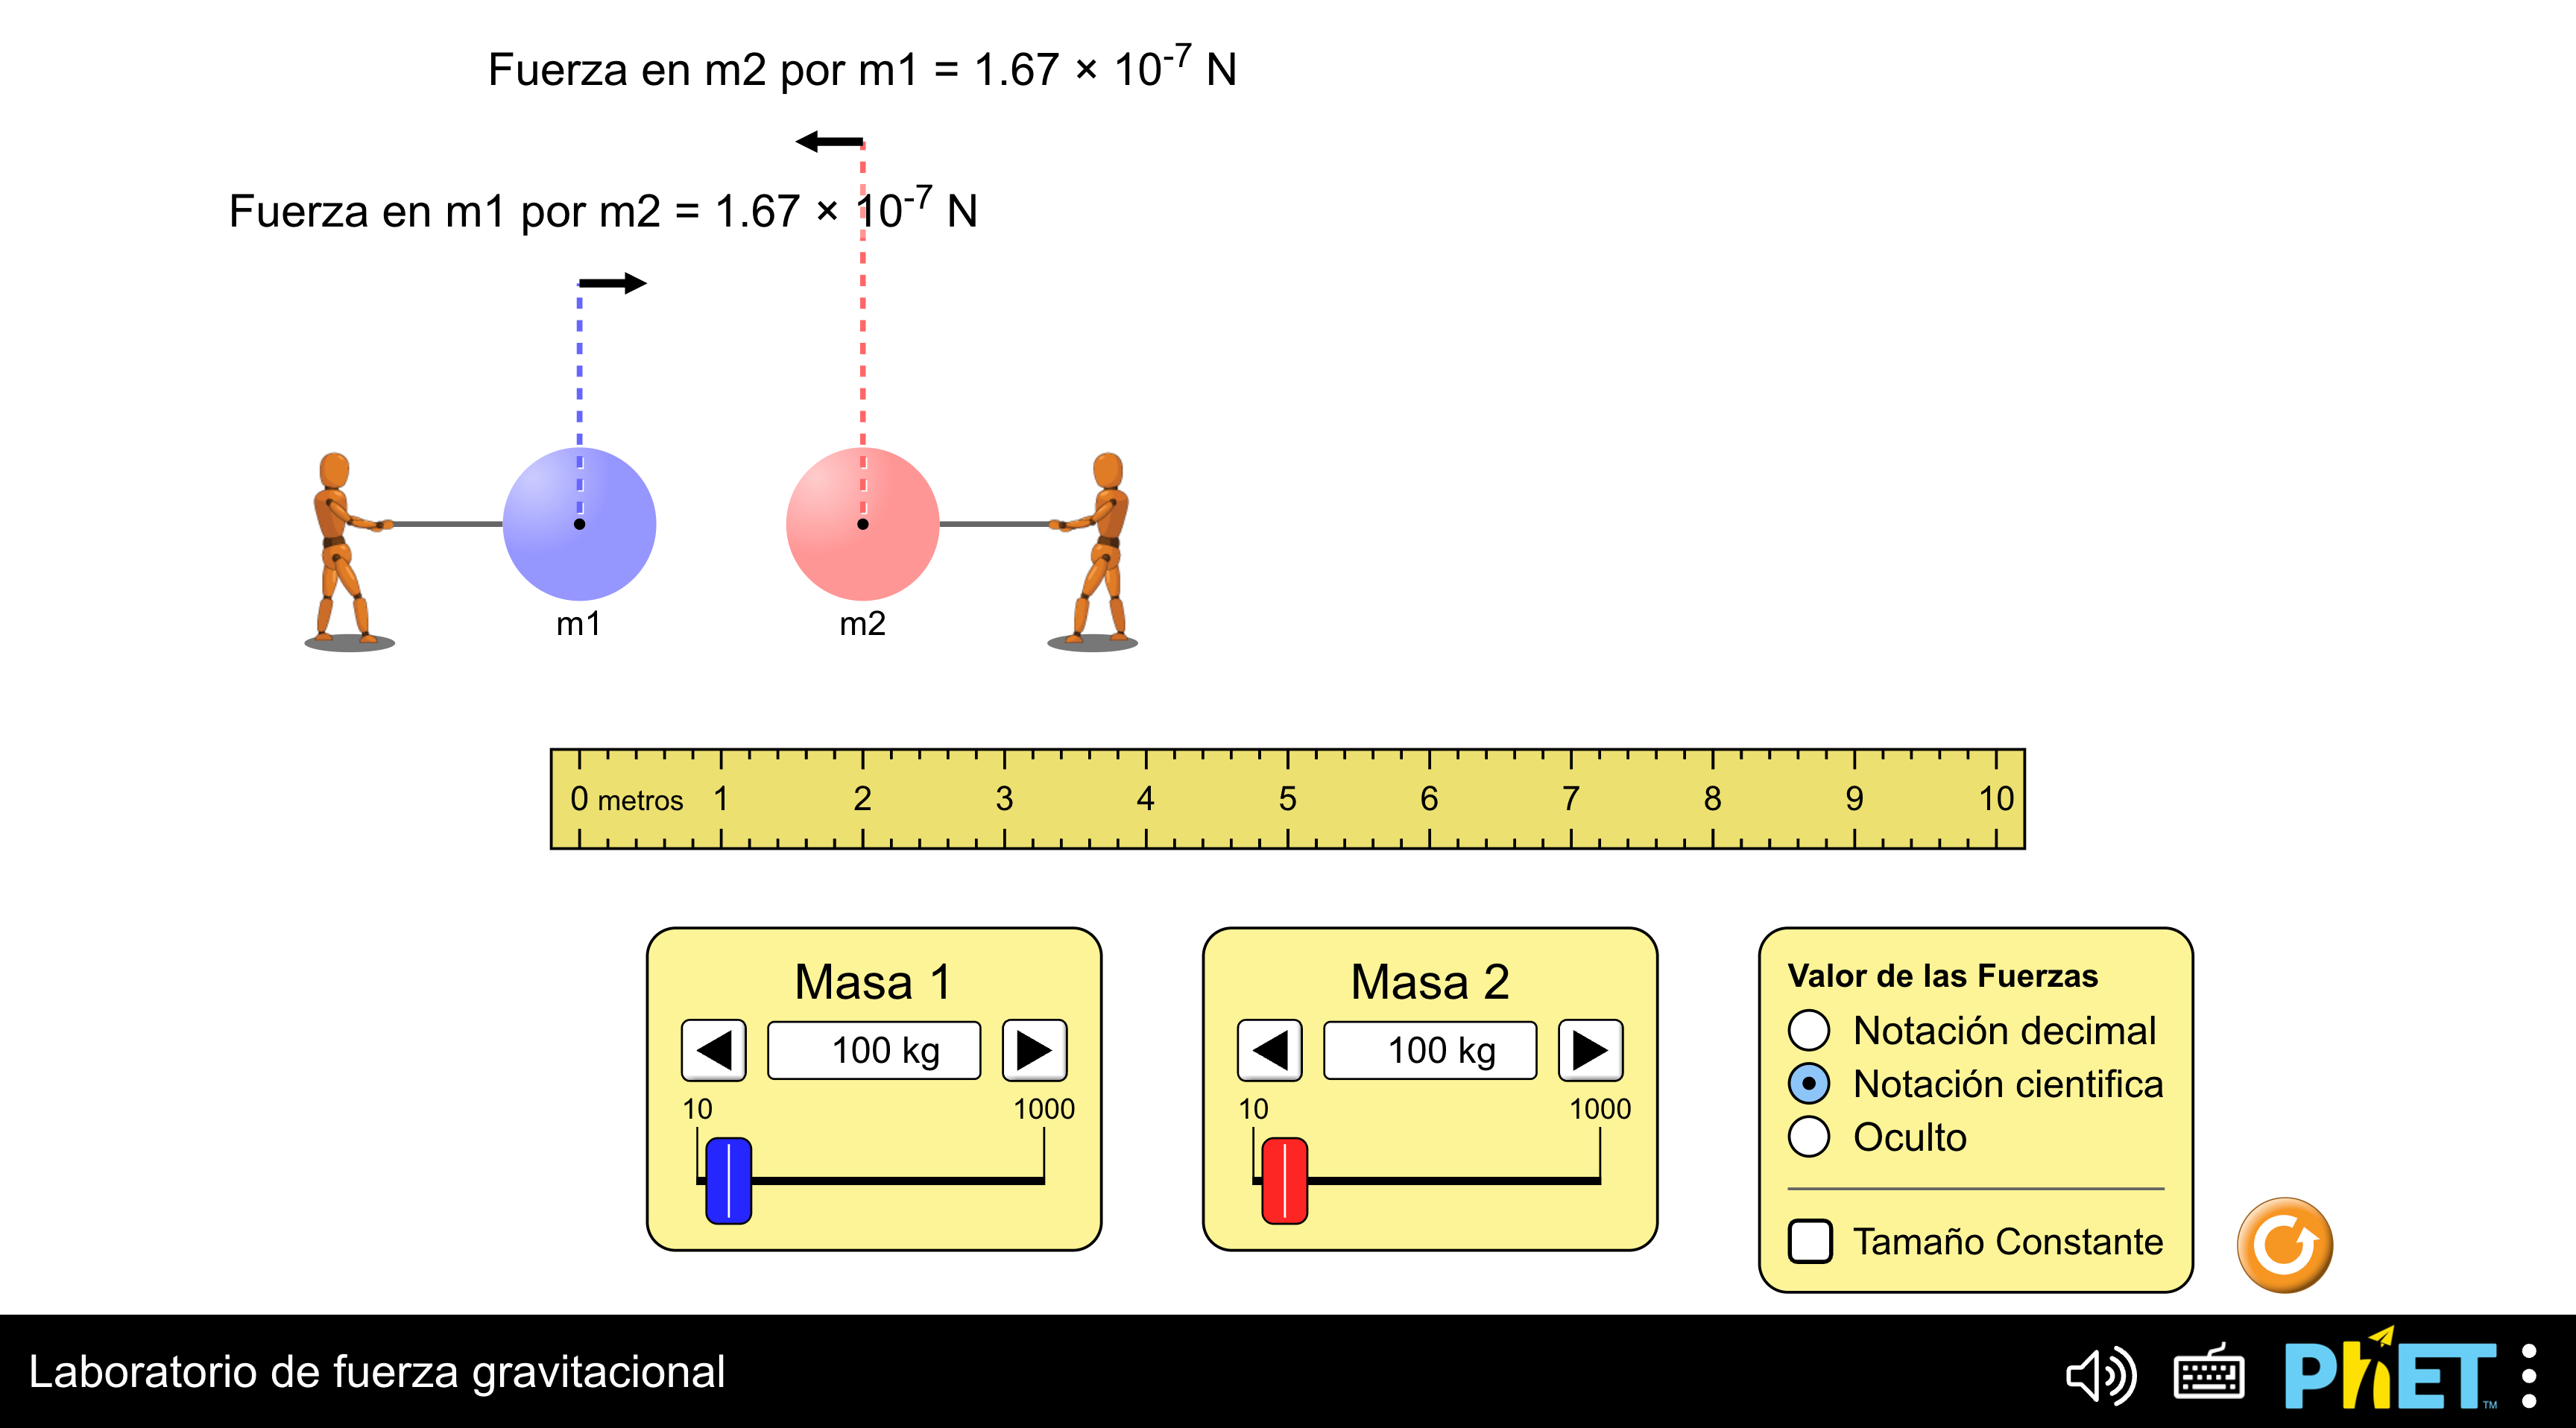
\includegraphics[width=0.55\linewidth]{m1_100_m2_100_r_2.png}
    \caption{Masa 100 kg vs Masa 100 kg, distancia de 2 m.}
    
    \vspace{0.5cm}

    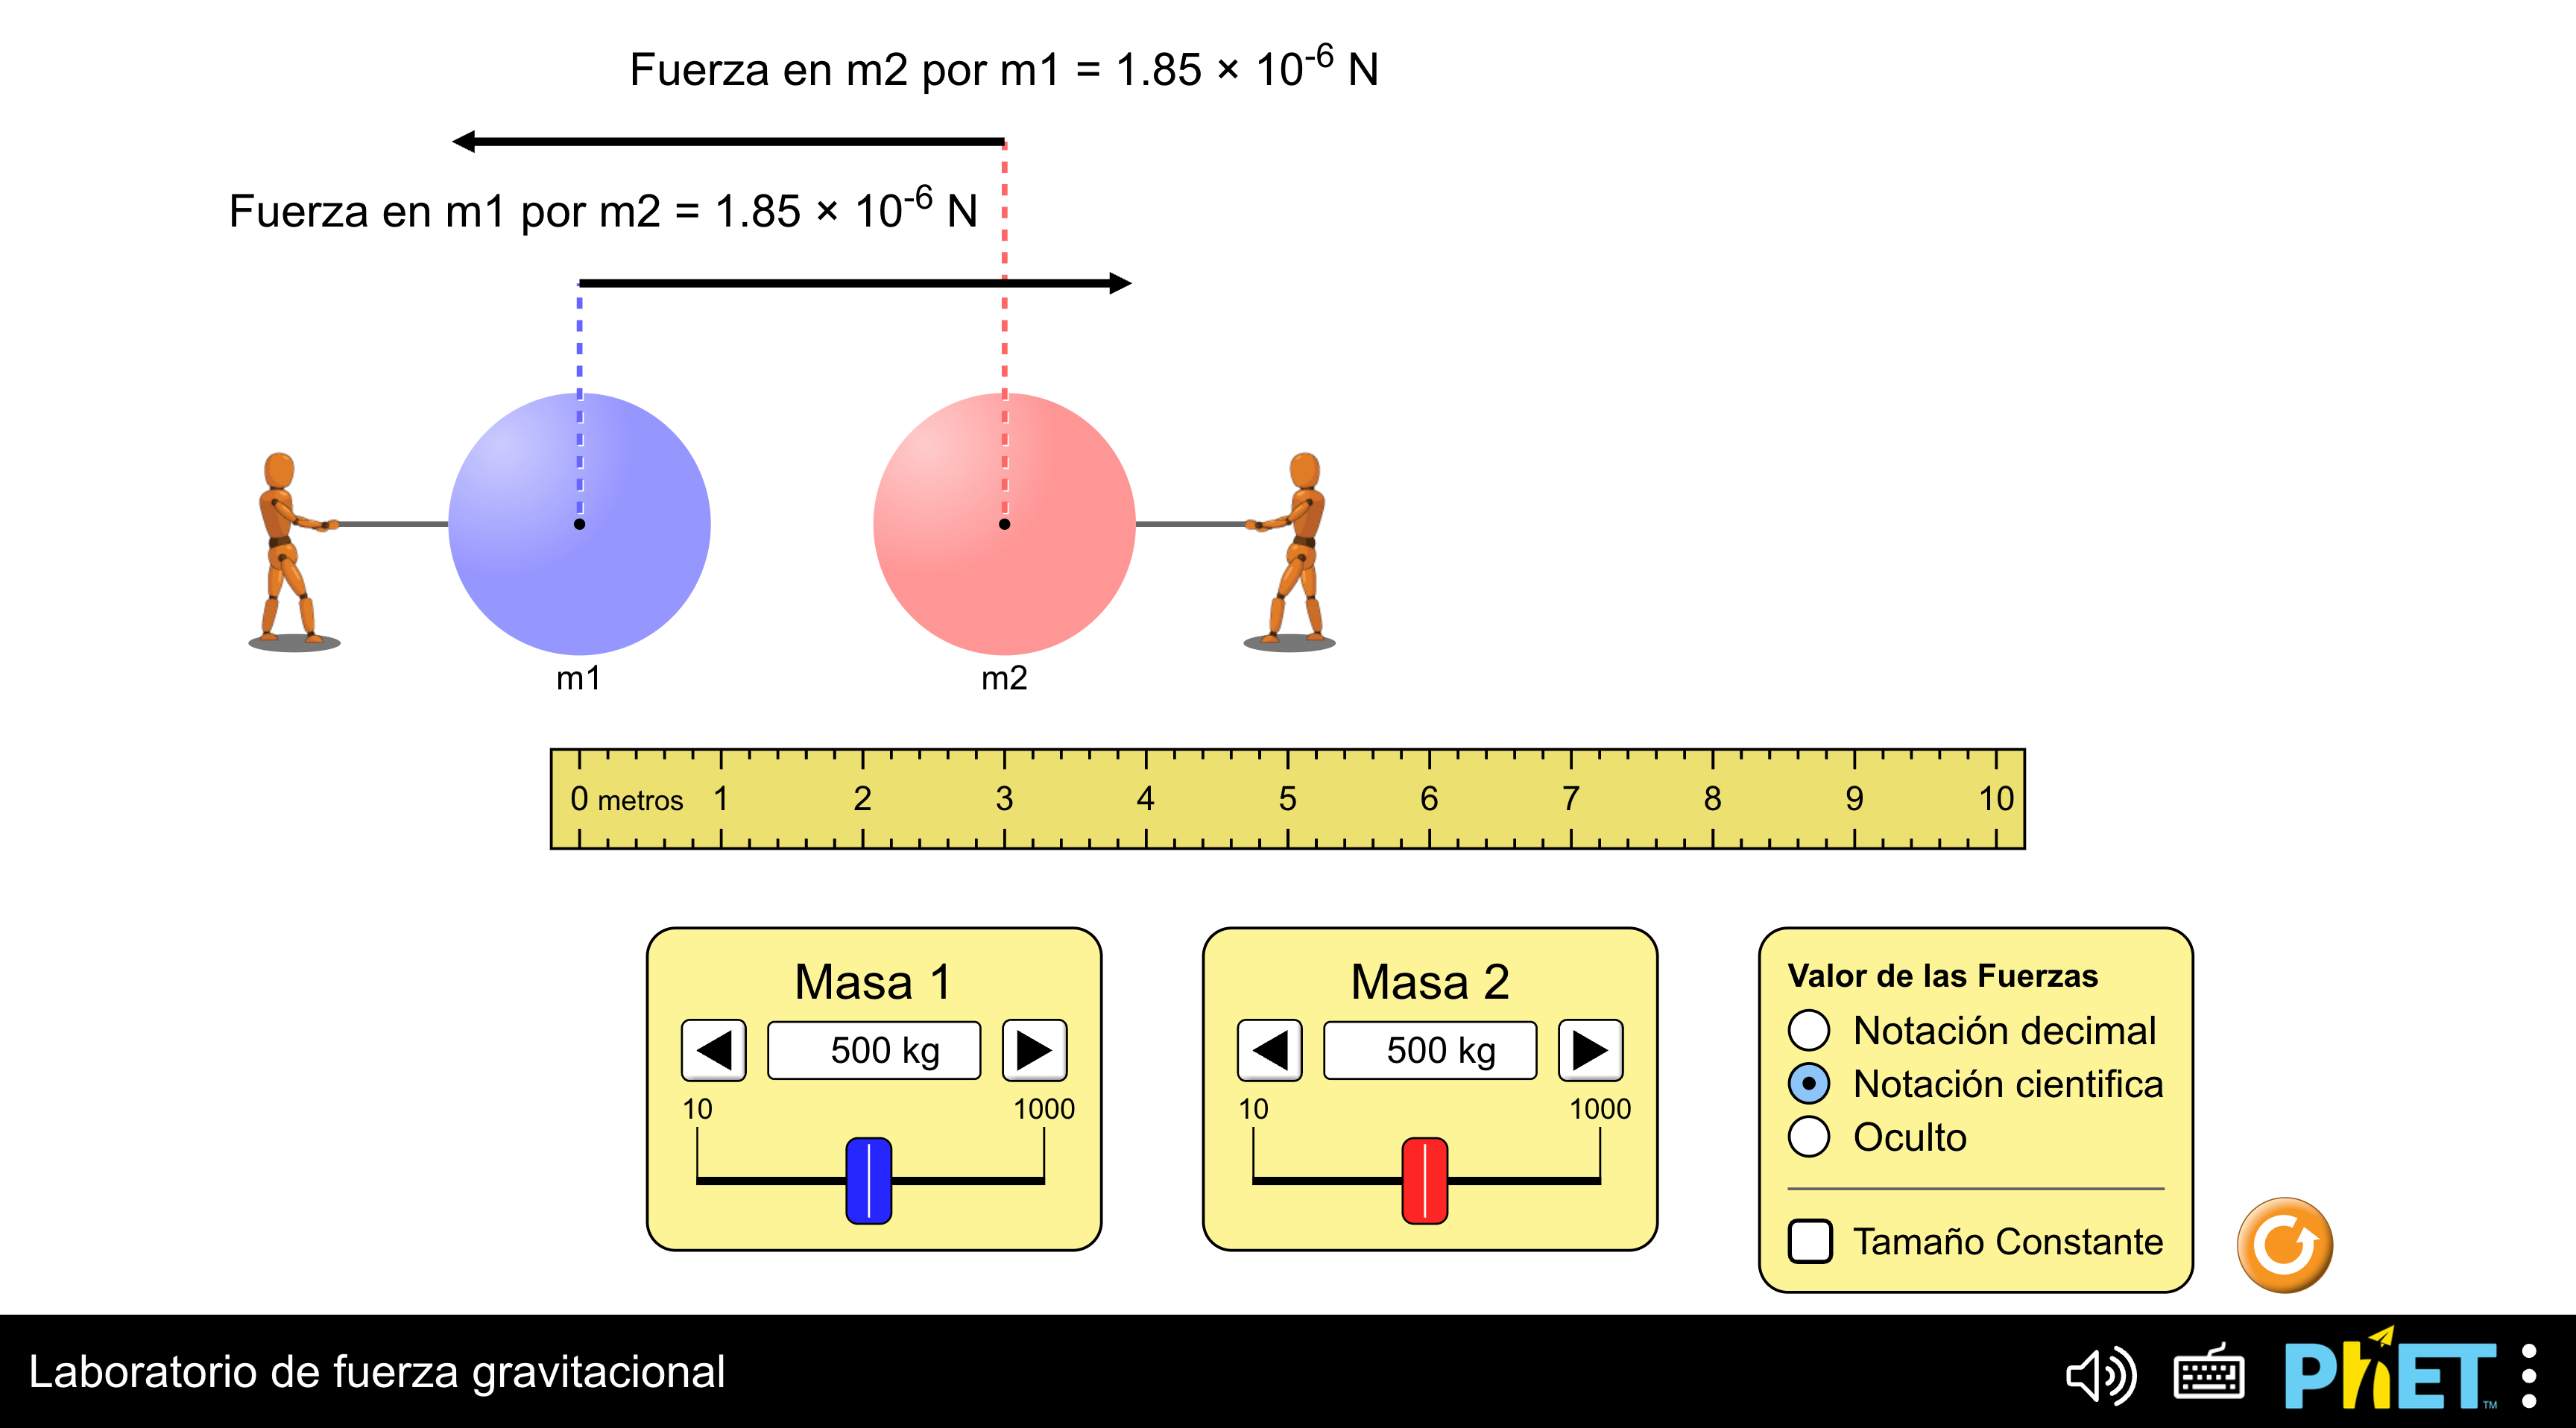
\includegraphics[width=0.55\linewidth]{m1_500_m2_500_r_3.png}
    \caption{Masa 500 kg vs Masa 500 kg, distancia de 3 m.}

    \vspace{0.5cm}

    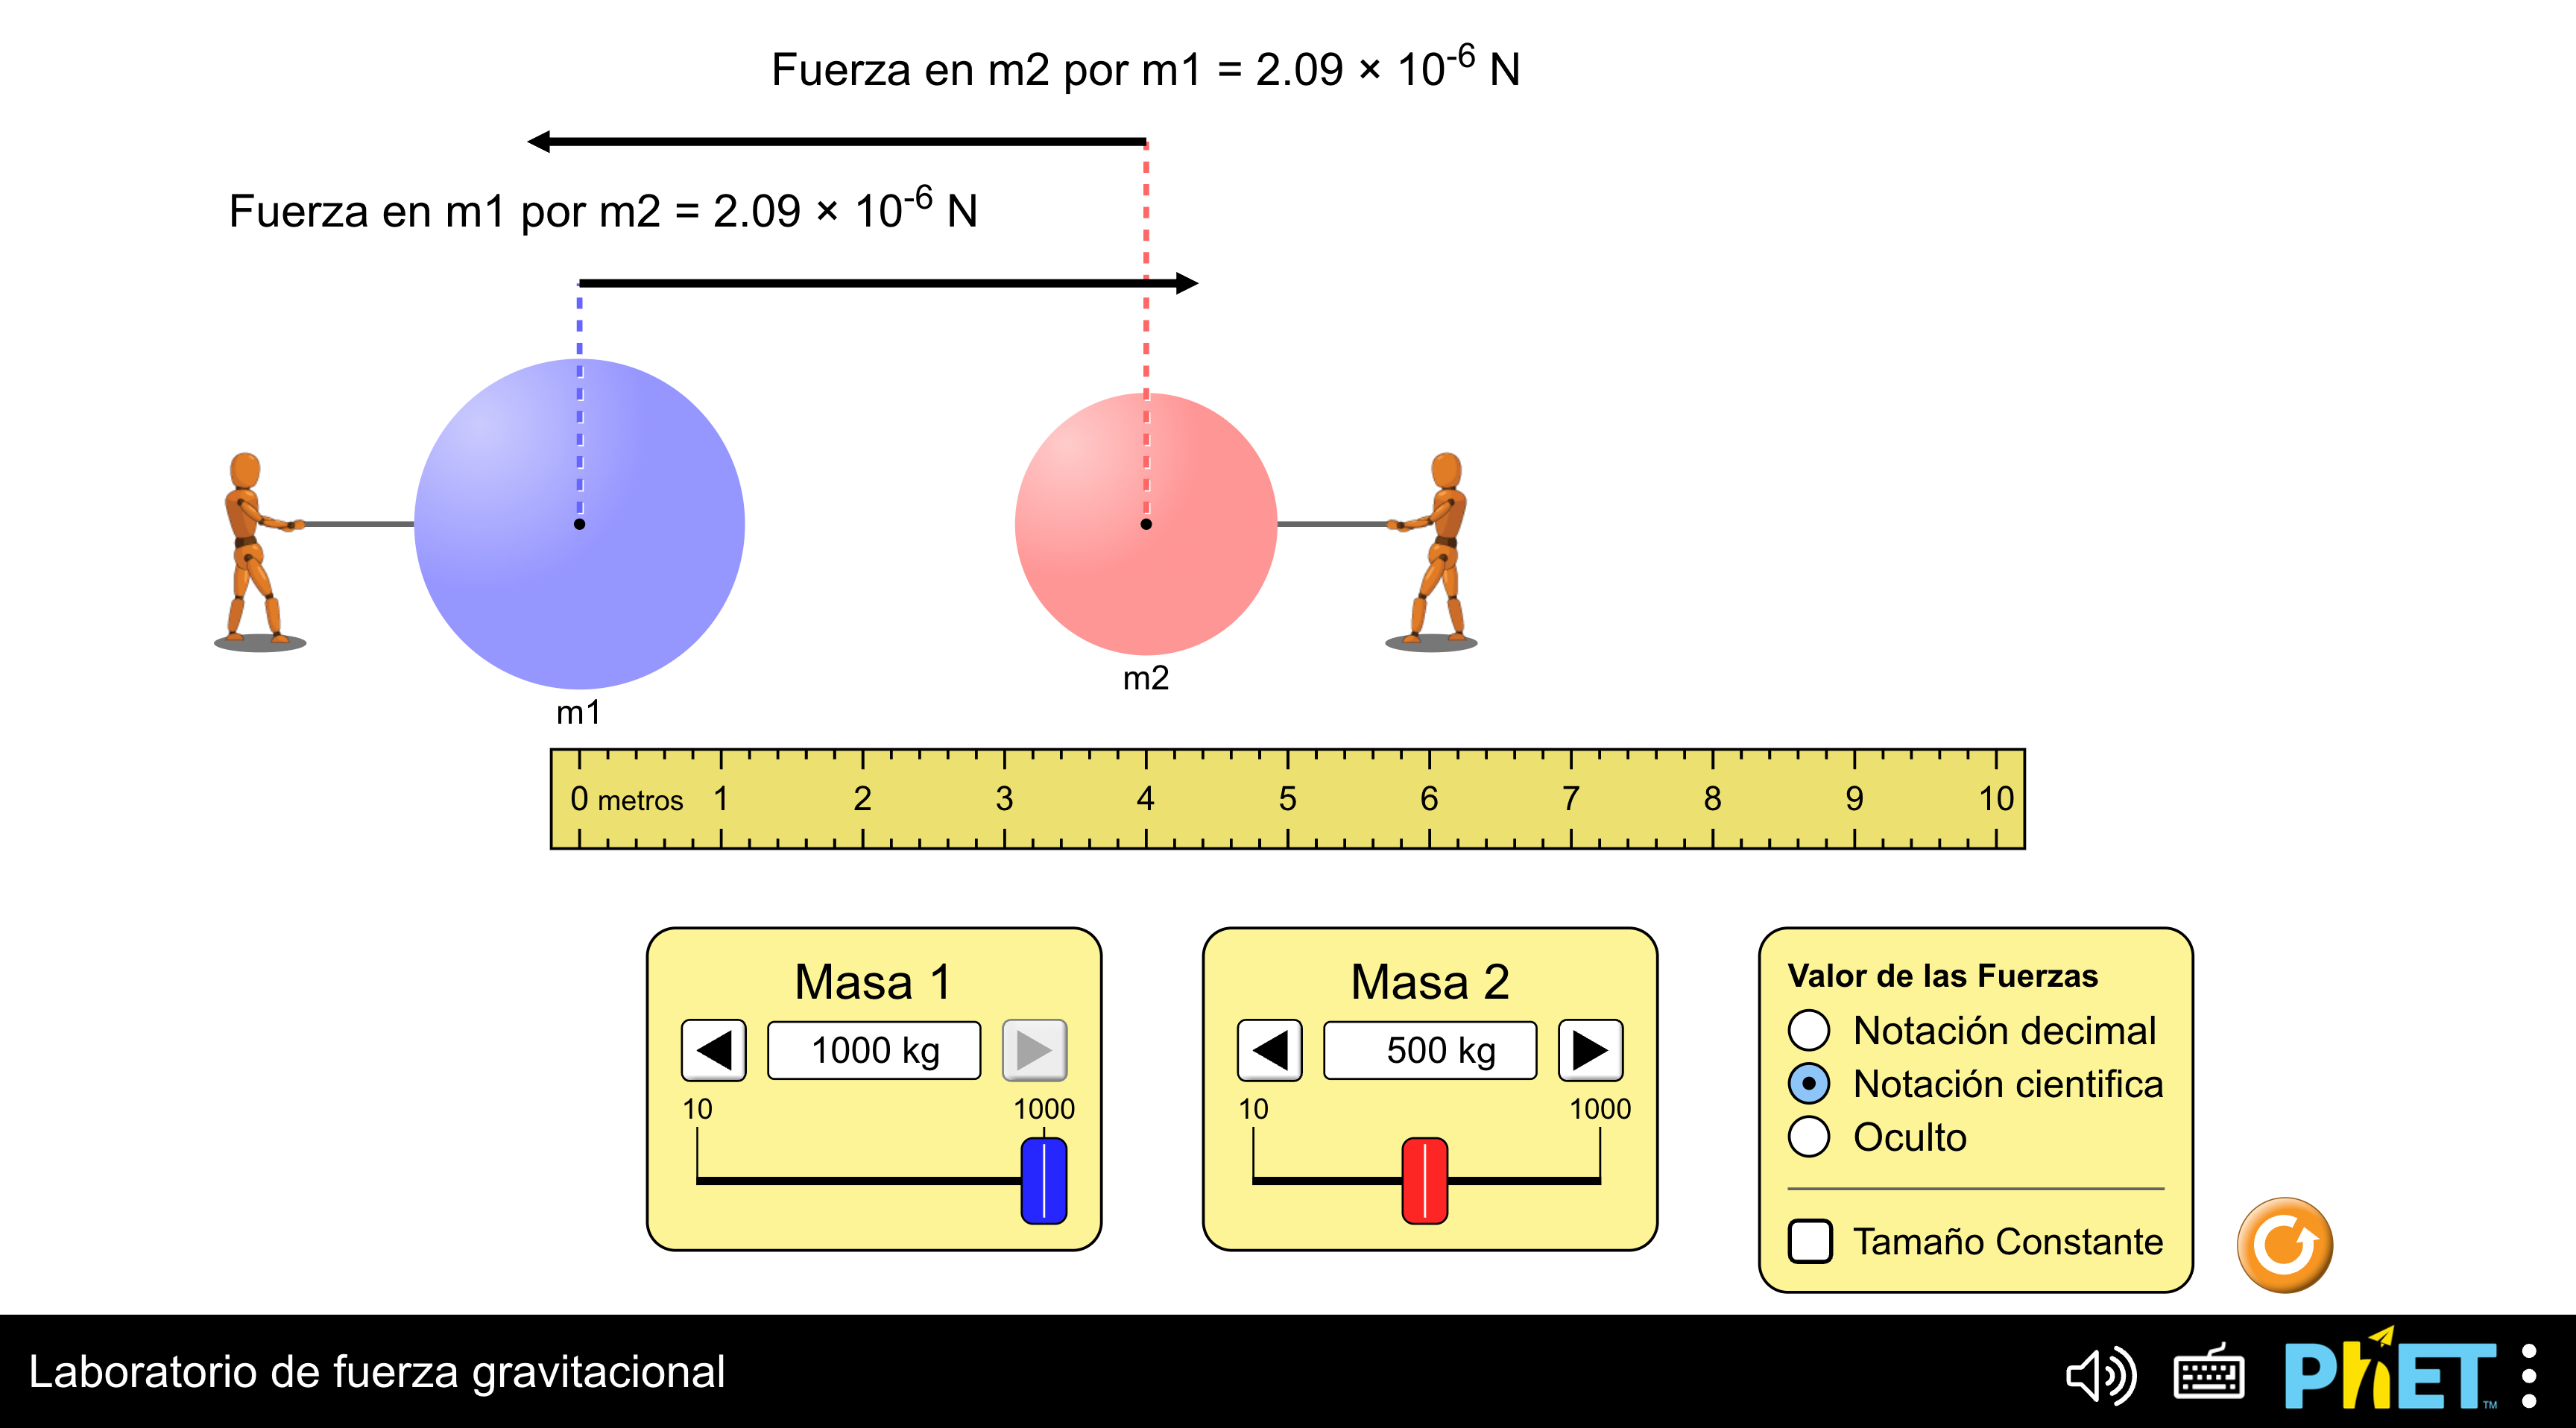
\includegraphics[width=0.55\linewidth]{m1_1000_m2_500_r_4.png}
    \caption{Masa 1000 kg vs Masa 500 kg, distancia de 4 m.}

\end{figure}

\newpage
\section{Análisis de Datos}
Los datos obtenidos se presentan en la Tabla \ref{tab:resultados}. Se compararon los valores observados con los valores teóricos calculados con la Ley de Gravitación Universal.


\begin{table}[h]
    \centering
    \renewcommand{\arraystretch}{1.3}
    \begin{tabular}{cccccc}
        \toprule
        \textbf{$m_1$ (kg)} & \textbf{$m_2$ (kg)} & \textbf{$r$ (m)} 
        & \textbf{$F_{obs}$ (N)} 
        & \textbf{$F_{teo}$ (N)} 
        & \textbf{Error (\%)} \\
        \midrule
        100  & 100  & 2  & $1.67 \times 10^{-7}$ & 0.000000167 (1.67$\times 10^{-7}$)  & 0.00 \\
        100  & 500  & 10 & $3.34 \times 10^{-8}$ & 0.0000000334 (3.34$\times 10^{-8}$) & 0.00 \\
        100  & 1000 & 7  & $1.36 \times 10^{-7}$ & 0.000000136 (1.36$\times 10^{-7}$)  & 0.00 \\
        500  & 100  & 9  & $4.12 \times 10^{-8}$ & 0.0000000412 (4.12$\times 10^{-8}$) & 0.00 \\
        500  & 500  & 3  & $1.85 \times 10^{-6}$ & 0.00000185 (1.85$\times 10^{-6}$)   & 0.00 \\
        500  & 1000 & 5  & $1.34 \times 10^{-6}$ & 0.00000133 (1.33$\times 10^{-6}$)   & 0.75 \\
        1000 & 100  & 8  & $1.04 \times 10^{-7}$ & 0.000000104 (1.04$\times 10^{-7}$)  & 0.00 \\
        1000 & 500  & 4  & $2.09 \times 10^{-6}$ & 0.00000208 (2.08$\times 10^{-6}$)   & 0.48 \\
        1000 & 1000 & 6  & $1.85 \times 10^{-6}$ & 0.00000185 (1.85$\times 10^{-6}$)   & 0.00 \\
        \bottomrule
    \end{tabular}
    \caption{Comparación entre la fuerza gravitacional observada y teórica.}
    \label{tab:resultados}
\end{table}

El análisis de los datos presentados en la Tabla~\ref{tab:resultados} evidencia que, en la mayoría de los casos, la fuerza observada coincide prácticamente con la fuerza teórica calculada mediante la Ley de Gravitación Universal de Newton. Con un error promedio del 0.0012\%, se concluye que la simulación de PhET es extremadamente precisa y confiable para el análisis de la fuerza gravitacional. Este resultado reafirma la validez del modelo teórico y destaca la eficacia de las herramientas de simulación en la enseñanza y estudio de fenómenos físicos.

\newpage
\section*{Cálculo de la Fuerza Teórica y Error Porcentual}

La fuerza teórica se calcula utilizando la Ley de Gravitación Universal, definida por la función:
\[
F_{\text{teo}}(m_1, m_2, r) = G\,\frac{m_1 \, m_2}{r^2}, \quad \text{donde} \quad G = 6.67 \times 10^{-11}\,\text{N}\,\text{m}^2/\text{kg}^2.
\]

El error porcentual entre la fuerza observada \(F_{\text{obs}}\) y la fuerza teórica \(F_{\text{teo}}\) se define como:
\[
\text{Error}(\%) = \left|\frac{F_{\text{obs}} - F_{\text{teo}}}{F_{\text{teo}}}\right| \times 100\%.
\]

Acontinuacion mostrare los calculos para dos de los ejemplos vistos en la tabla anterior

\subsection*{Caso 1: masa de 100 kg vs masa de 100 kg, distancia de 2 m}

\textbf{Datos:}
\[
m_1 = 100\,\text{kg}, \quad m_2 = 100\,\text{kg}, \quad r = 2\,\text{m}, \quad F_{\text{obs}} = 1.67 \times 10^{-7}\,\text{N}.
\]

\textbf{Cálculo de \(F_{\text{teo}}\):}
\begin{align*}
F_{\text{teo}} &= 6.67 \times 10^{-11}\,\frac{100 \times 100}{2^2} \\
               &= 6.67 \times 10^{-11}\,\frac{10\,000}{4} \\
               &= 6.67 \times 10^{-11} \times 2500 \\
               &= 1.6675 \times 10^{-7}\,\text{N} \\
               &\approx 1.67 \times 10^{-7}\,\text{N}.
\end{align*}

\textbf{Cálculo del error:}
\[
\text{Error}(\%) = \left|\frac{1.67 \times 10^{-7} - 1.67 \times 10^{-7}}{1.67 \times 10^{-7}}\right| \times 100\% = 0\%.
\]

En este caso, \(F_{\text{obs}} = F_{\text{teo}}\), por lo que el error es 0\%.

\subsection*{Caso 2: masa de 500 kg vs masa de 1000 kg, distancia de 5 m}

\textbf{Datos:}
\[
m_1 = 500\,\text{kg}, \quad m_2 = 1000\,\text{kg}, \quad r = 5\,\text{m}, \quad F_{\text{obs}} = 1.34 \times 10^{-6}\,\text{N}.
\]

\textbf{Cálculo de \(F_{\text{teo}}\):}
\begin{align*}
F_{\text{teo}} &= 6.67 \times 10^{-11}\,\frac{500 \times 1000}{5^2} \\
               &= 6.67 \times 10^{-11}\,\frac{500\,000}{25} \\
               &= 6.67 \times 10^{-11} \times 20\,000 \\
               &= 1.334 \times 10^{-6}\,\text{N} \\
               &\approx 1.33 \times 10^{-6}\,\text{N}.
\end{align*}

\textbf{Cálculo del error:}
\begin{align*}
\Delta F &= F_{\text{obs}} - F_{\text{teo}} = 1.34 \times 10^{-6} - 1.33 \times 10^{-6} = 1.0 \times 10^{-8}\,\text{N}, \\
\text{Error}(\%) &= \left|\frac{1.0 \times 10^{-8}}{1.33 \times 10^{-6}}\right| \times 100\% \approx 0.75\%.
\end{align*}

En este caso se observa un pequeño margen de error, ya que \(F_{\text{obs}}\) es ligeramente mayor que \(F_{\text{teo}}\).


\newpage
\section*{Conclusión}

En este ejercicio se aplicó la Ley de Gravitación Universal para calcular la fuerza teórica entre dos masas y se comparó con los valores obtenidos experimentalmente. Se pudo observar que, en la mayoría de los casos, la fuerza observada coincide prácticamente con la fuerza teórica, lo que confirma la validez y precisión del modelo teórico en la descripción de la interacción gravitacional.

El pequeño margen de error encontrado en uno de los casos (aproximadamente 0.75\%) sugiere que, aunque el modelo es robusto, pueden existir leves discrepancias atribuibles a imprecisiones en las mediciones experimentales, redondeos o condiciones experimentales particulares. Esto resalta la importancia de considerar y cuantificar los errores en cualquier estudio experimental para una comparación precisa con las predicciones teóricas.

En resumen, el ejercicio no solo reafirma la utilidad de la Ley de Gravitación Universal para predecir fuerzas en sistemas físicos, sino que también enfatiza la relevancia de un análisis crítico y detallado de los datos experimentales frente a los modelos teóricos.

\newpage
\begin{thebibliography}{9}
    \bibitem{fisicalab}
    FísicaLab. \textit{Ley de Gravitación Universal}. Disponible en: \url{https://www.fisicalab.com/apartado/ley-gravitacion-universal}.
    
    \bibitem{latexhelp}
    LaTeX Project. \textit{Help}. Disponible en: \url{https://www.latex-project.org/help/}.
    
    \bibitem{phet}
    PhET Interactive Simulations. \textit{Gravity Force Lab}. Disponible en: \url{https://phet.colorado.edu/es_PE/simulations/gravity-force-lab/about?locale=es_CO}.
\end{thebibliography}

\newpage
\section*{Enlaces}
Para mayor información y recursos adicionales, consulte:
\begin{itemize}
    \item \textbf{Repositorio en GitHub:} \url{https://github.com/jcamilofarfan/ACA_Fisica_Mecanica_y_Laboratorio}
    \item \textbf{Video Explicativo:} \url{https://drive.google.com/file/d/1jCZoUOUDmyrEAqy0wWHw_v8tBPJuKyxR/view?usp=sharing}
\end{itemize}

\newpage
\section{Anexos}
A continuación se muestran todas las imágenes del experimento:

\begin{figure}[h]
    \centering
    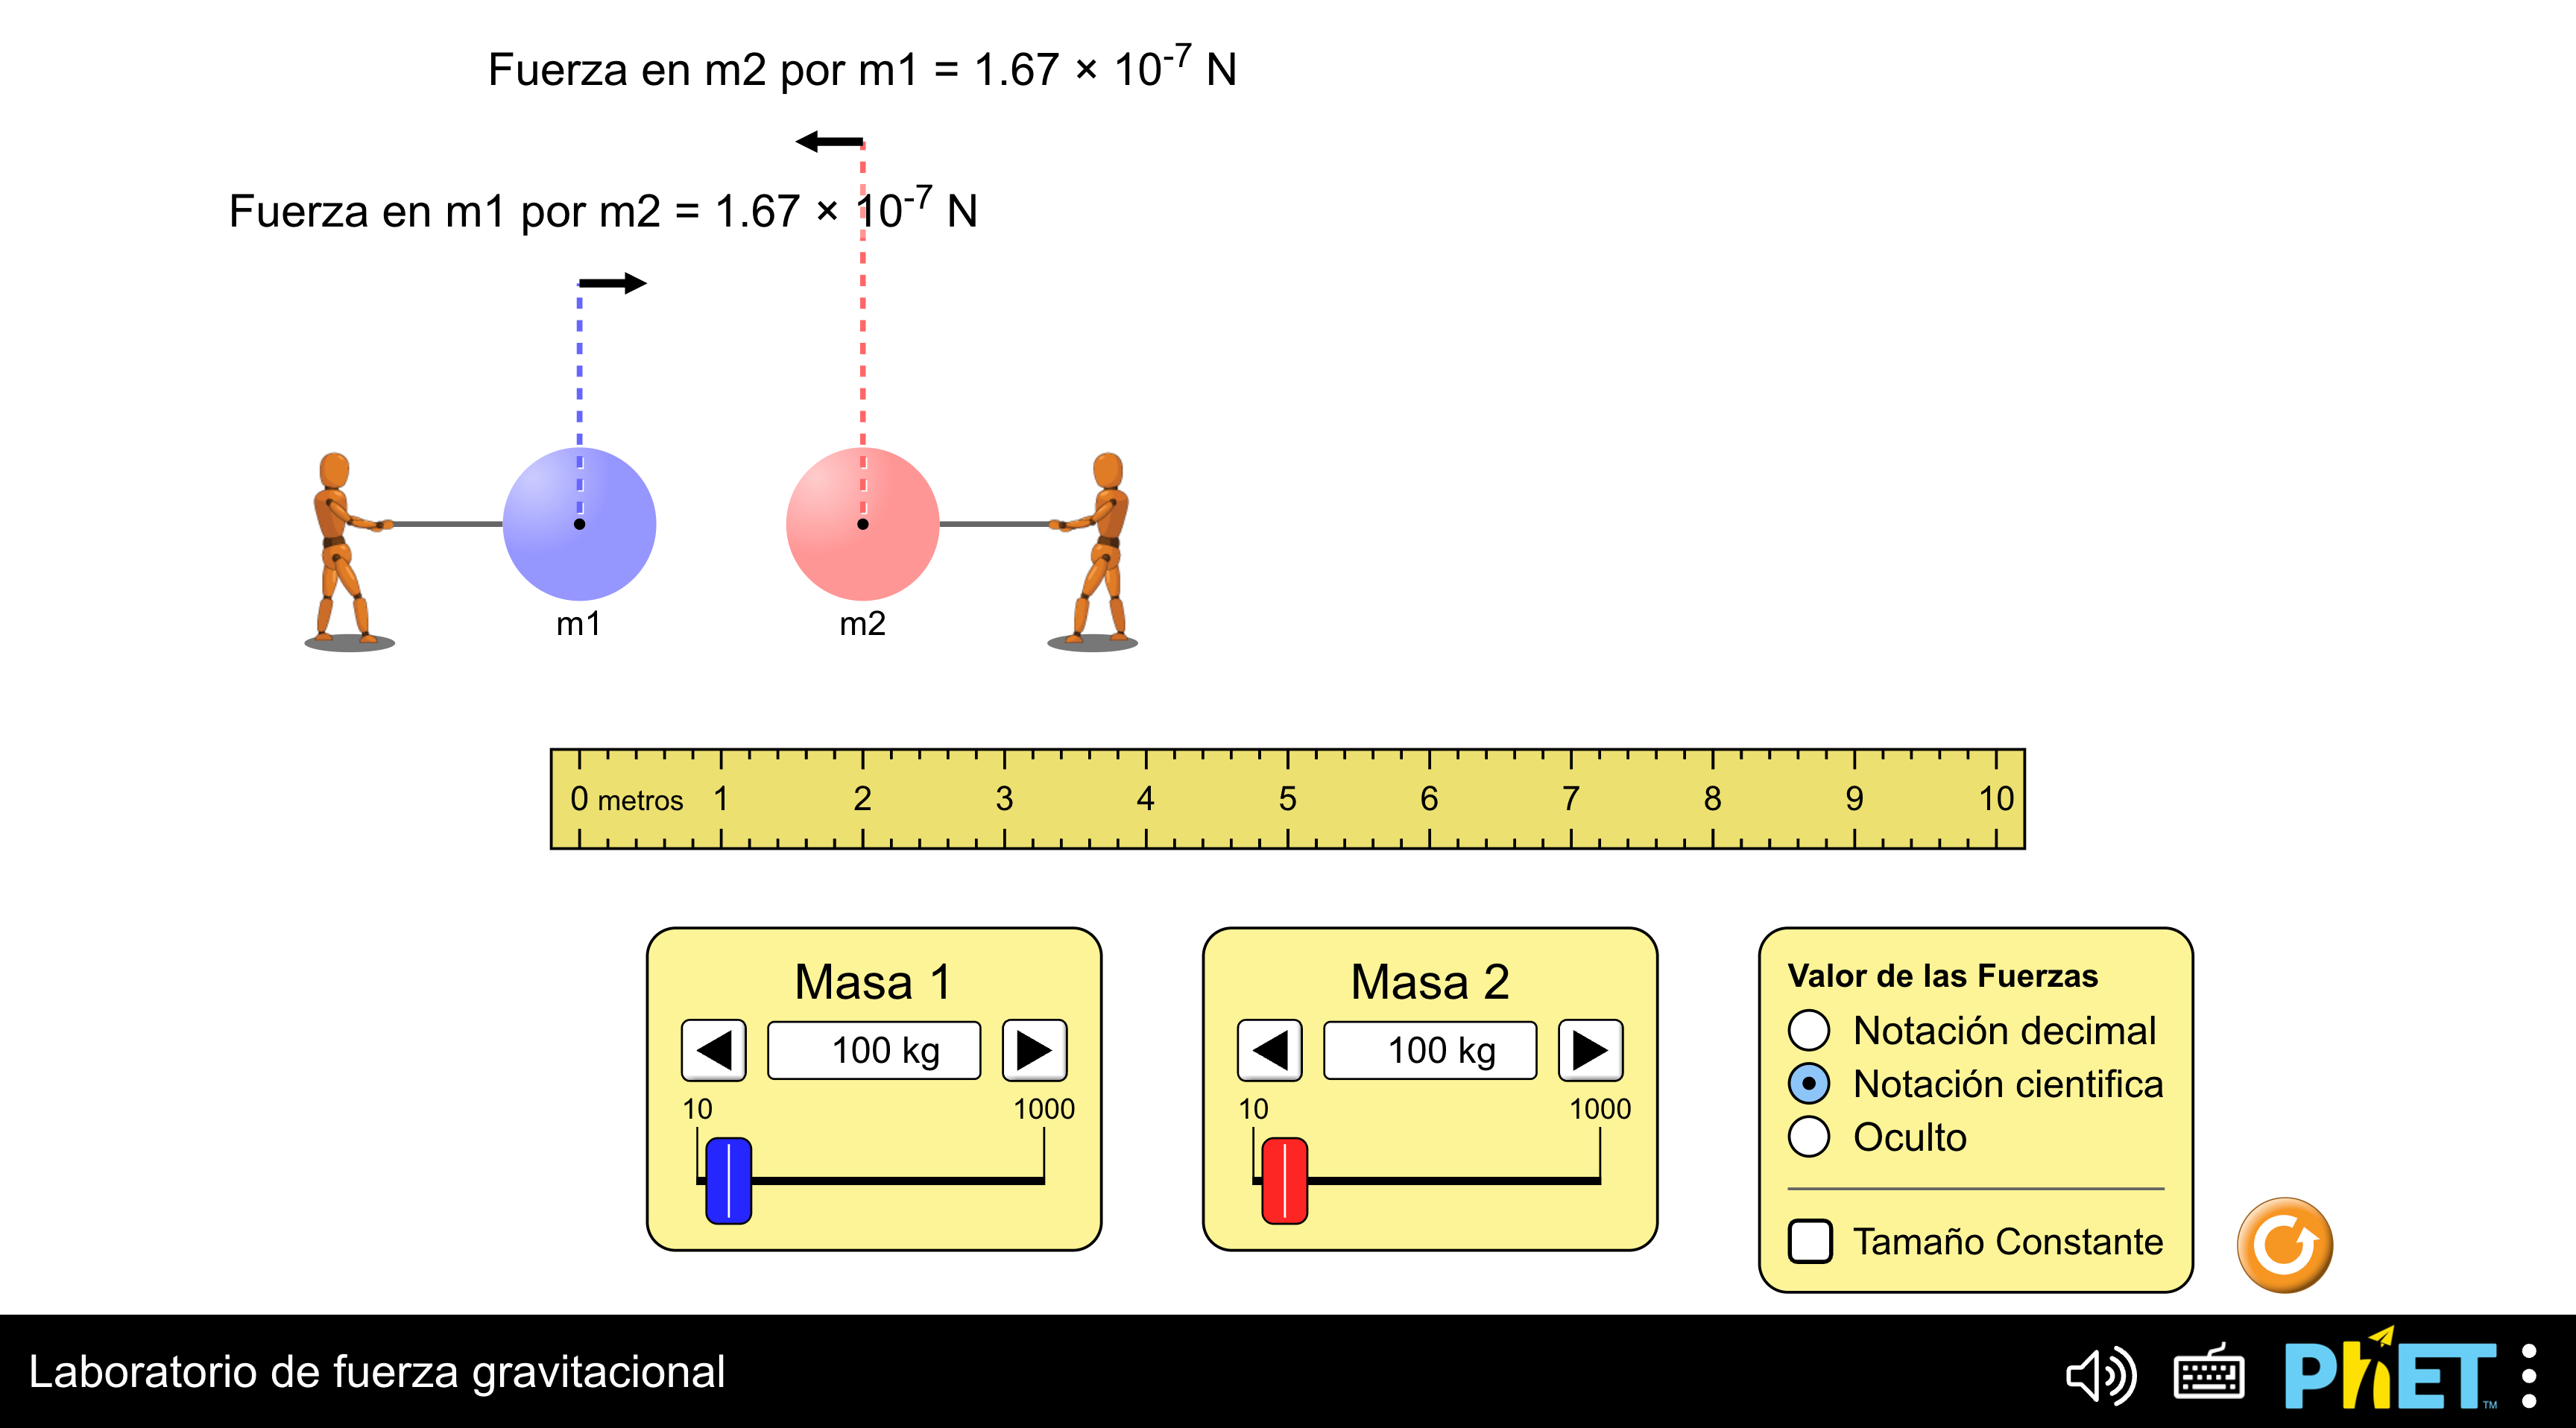
\includegraphics[width=1\linewidth]{m1_100_m2_100_r_2.png}
    \caption{Masa 100 kg vs Masa 100 kg, distancia de 2 m.}
\end{figure}

\begin{figure}[h]
    \centering
    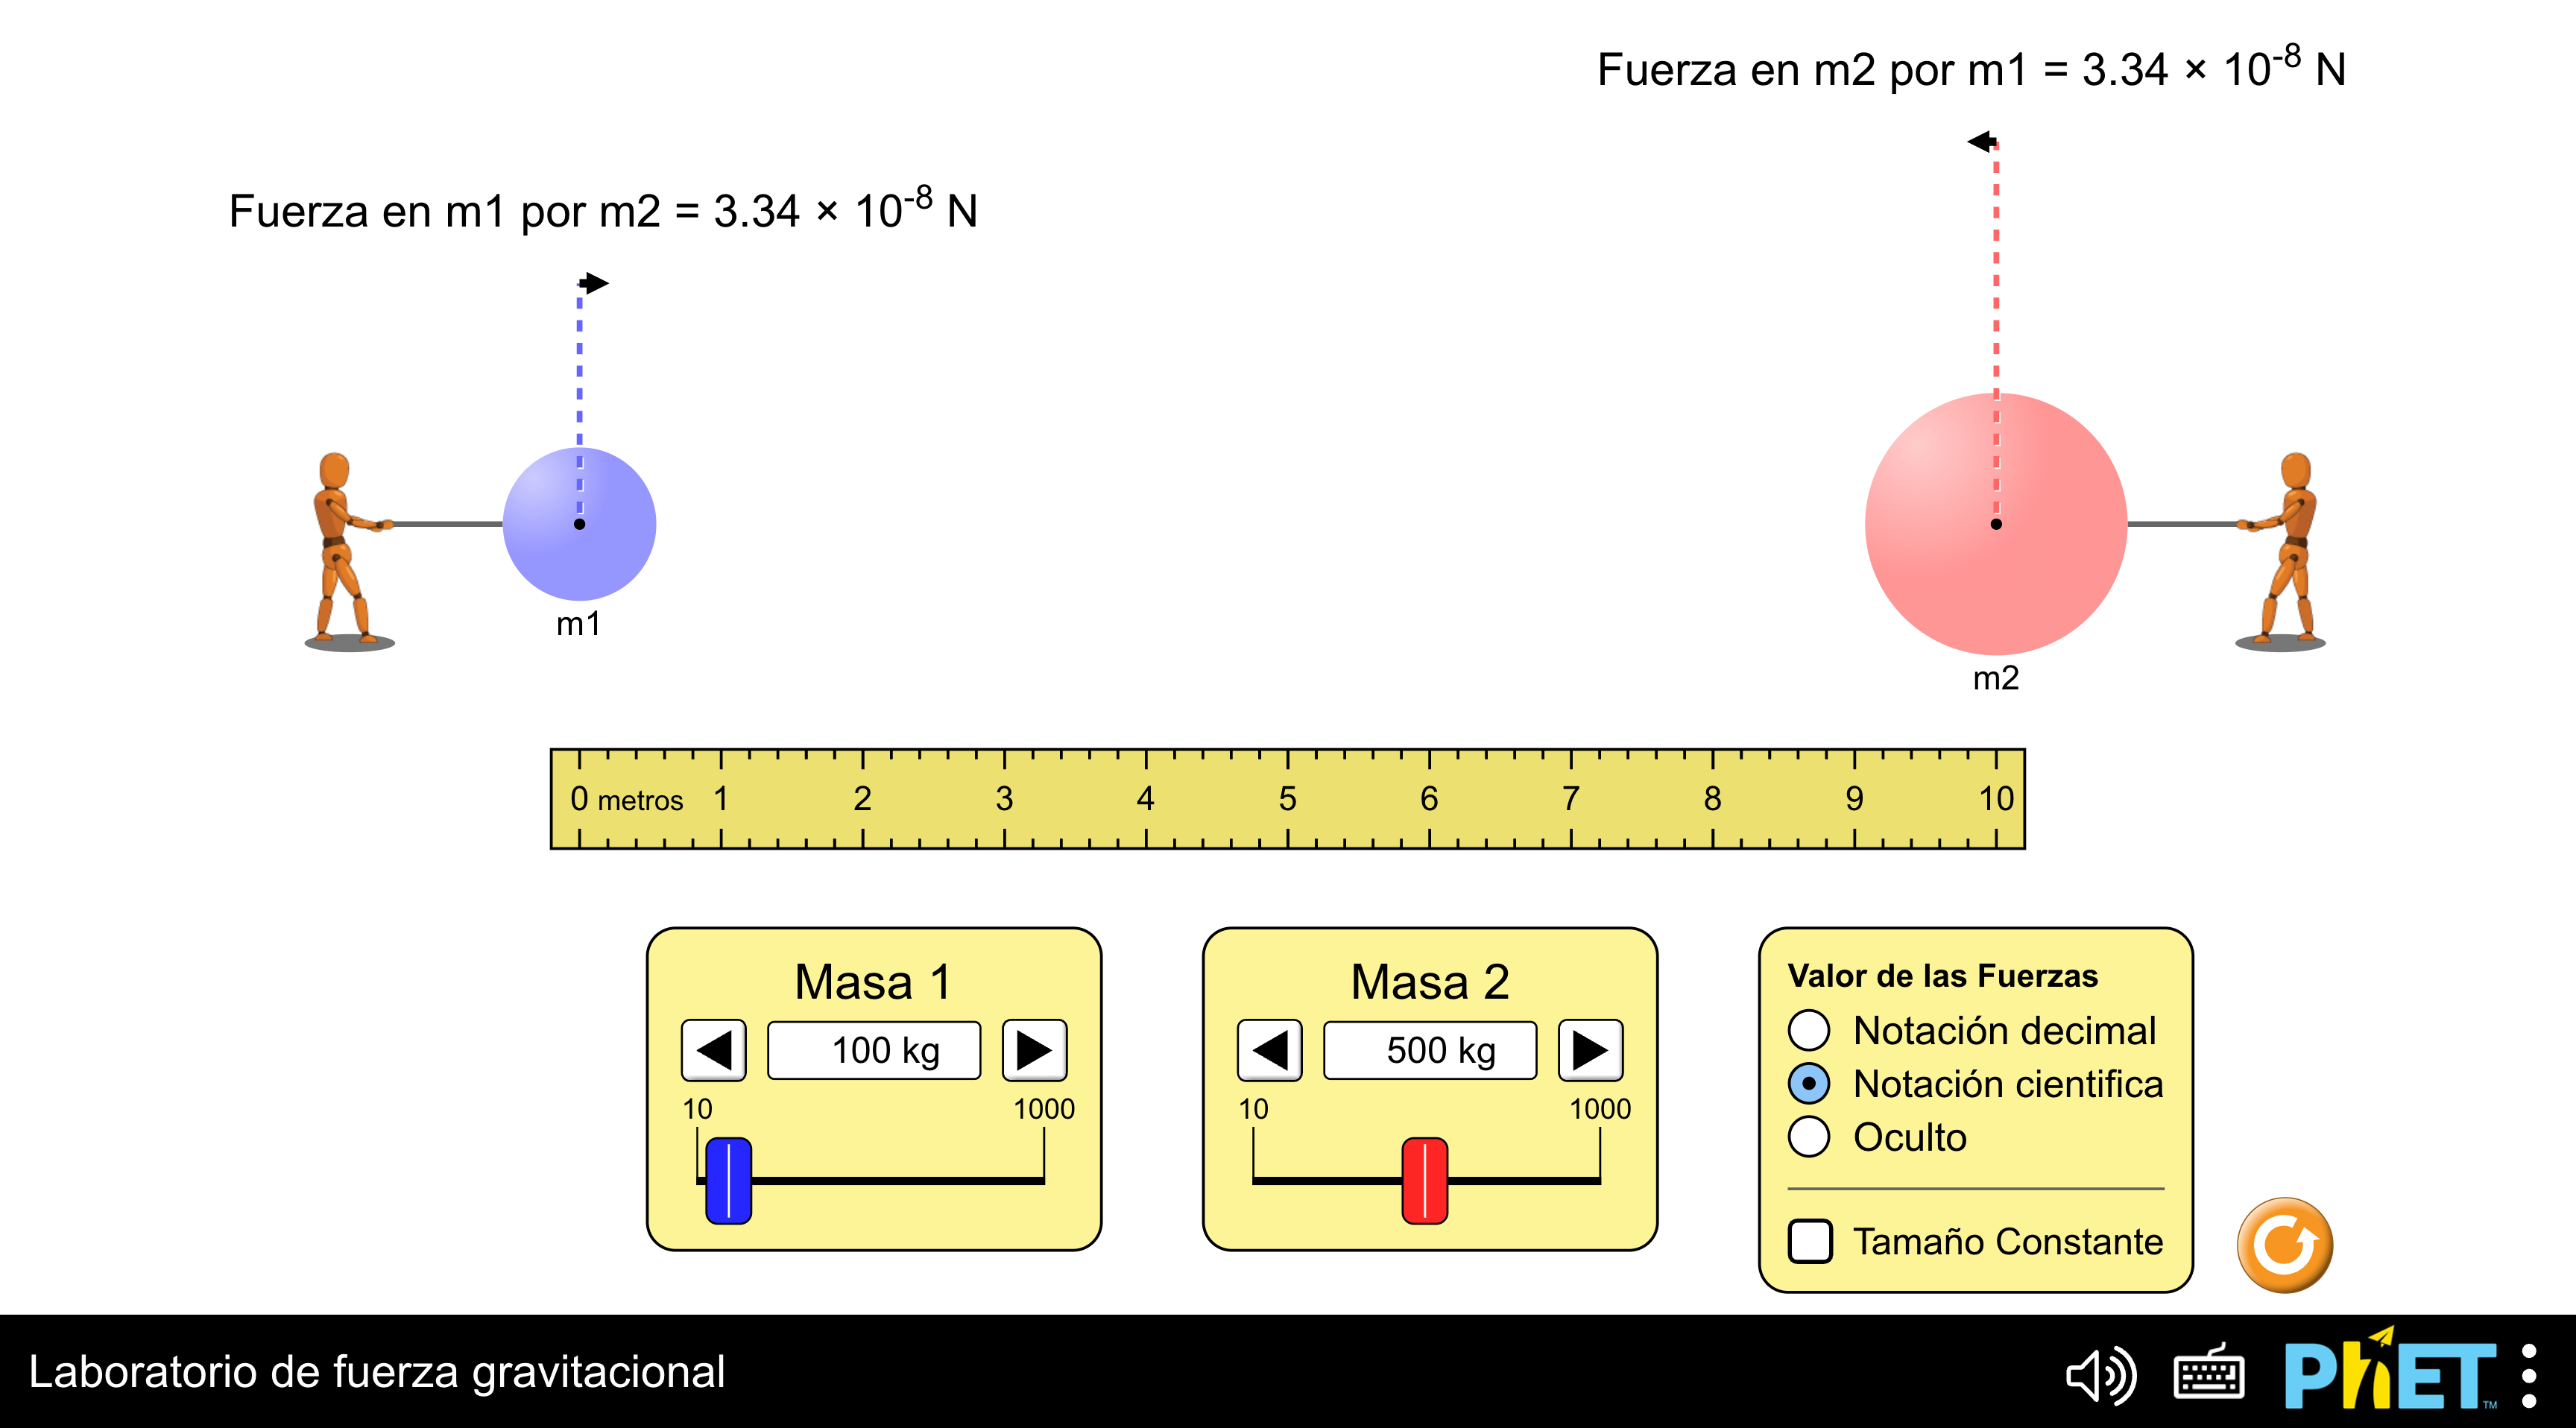
\includegraphics[width=1\linewidth]{m1_100_m2_500_r_10.png}
    \caption{Masa 100 kg vs Masa 500 kg, distancia de 10 m.}
\end{figure}

\begin{figure}[h]
    \centering
    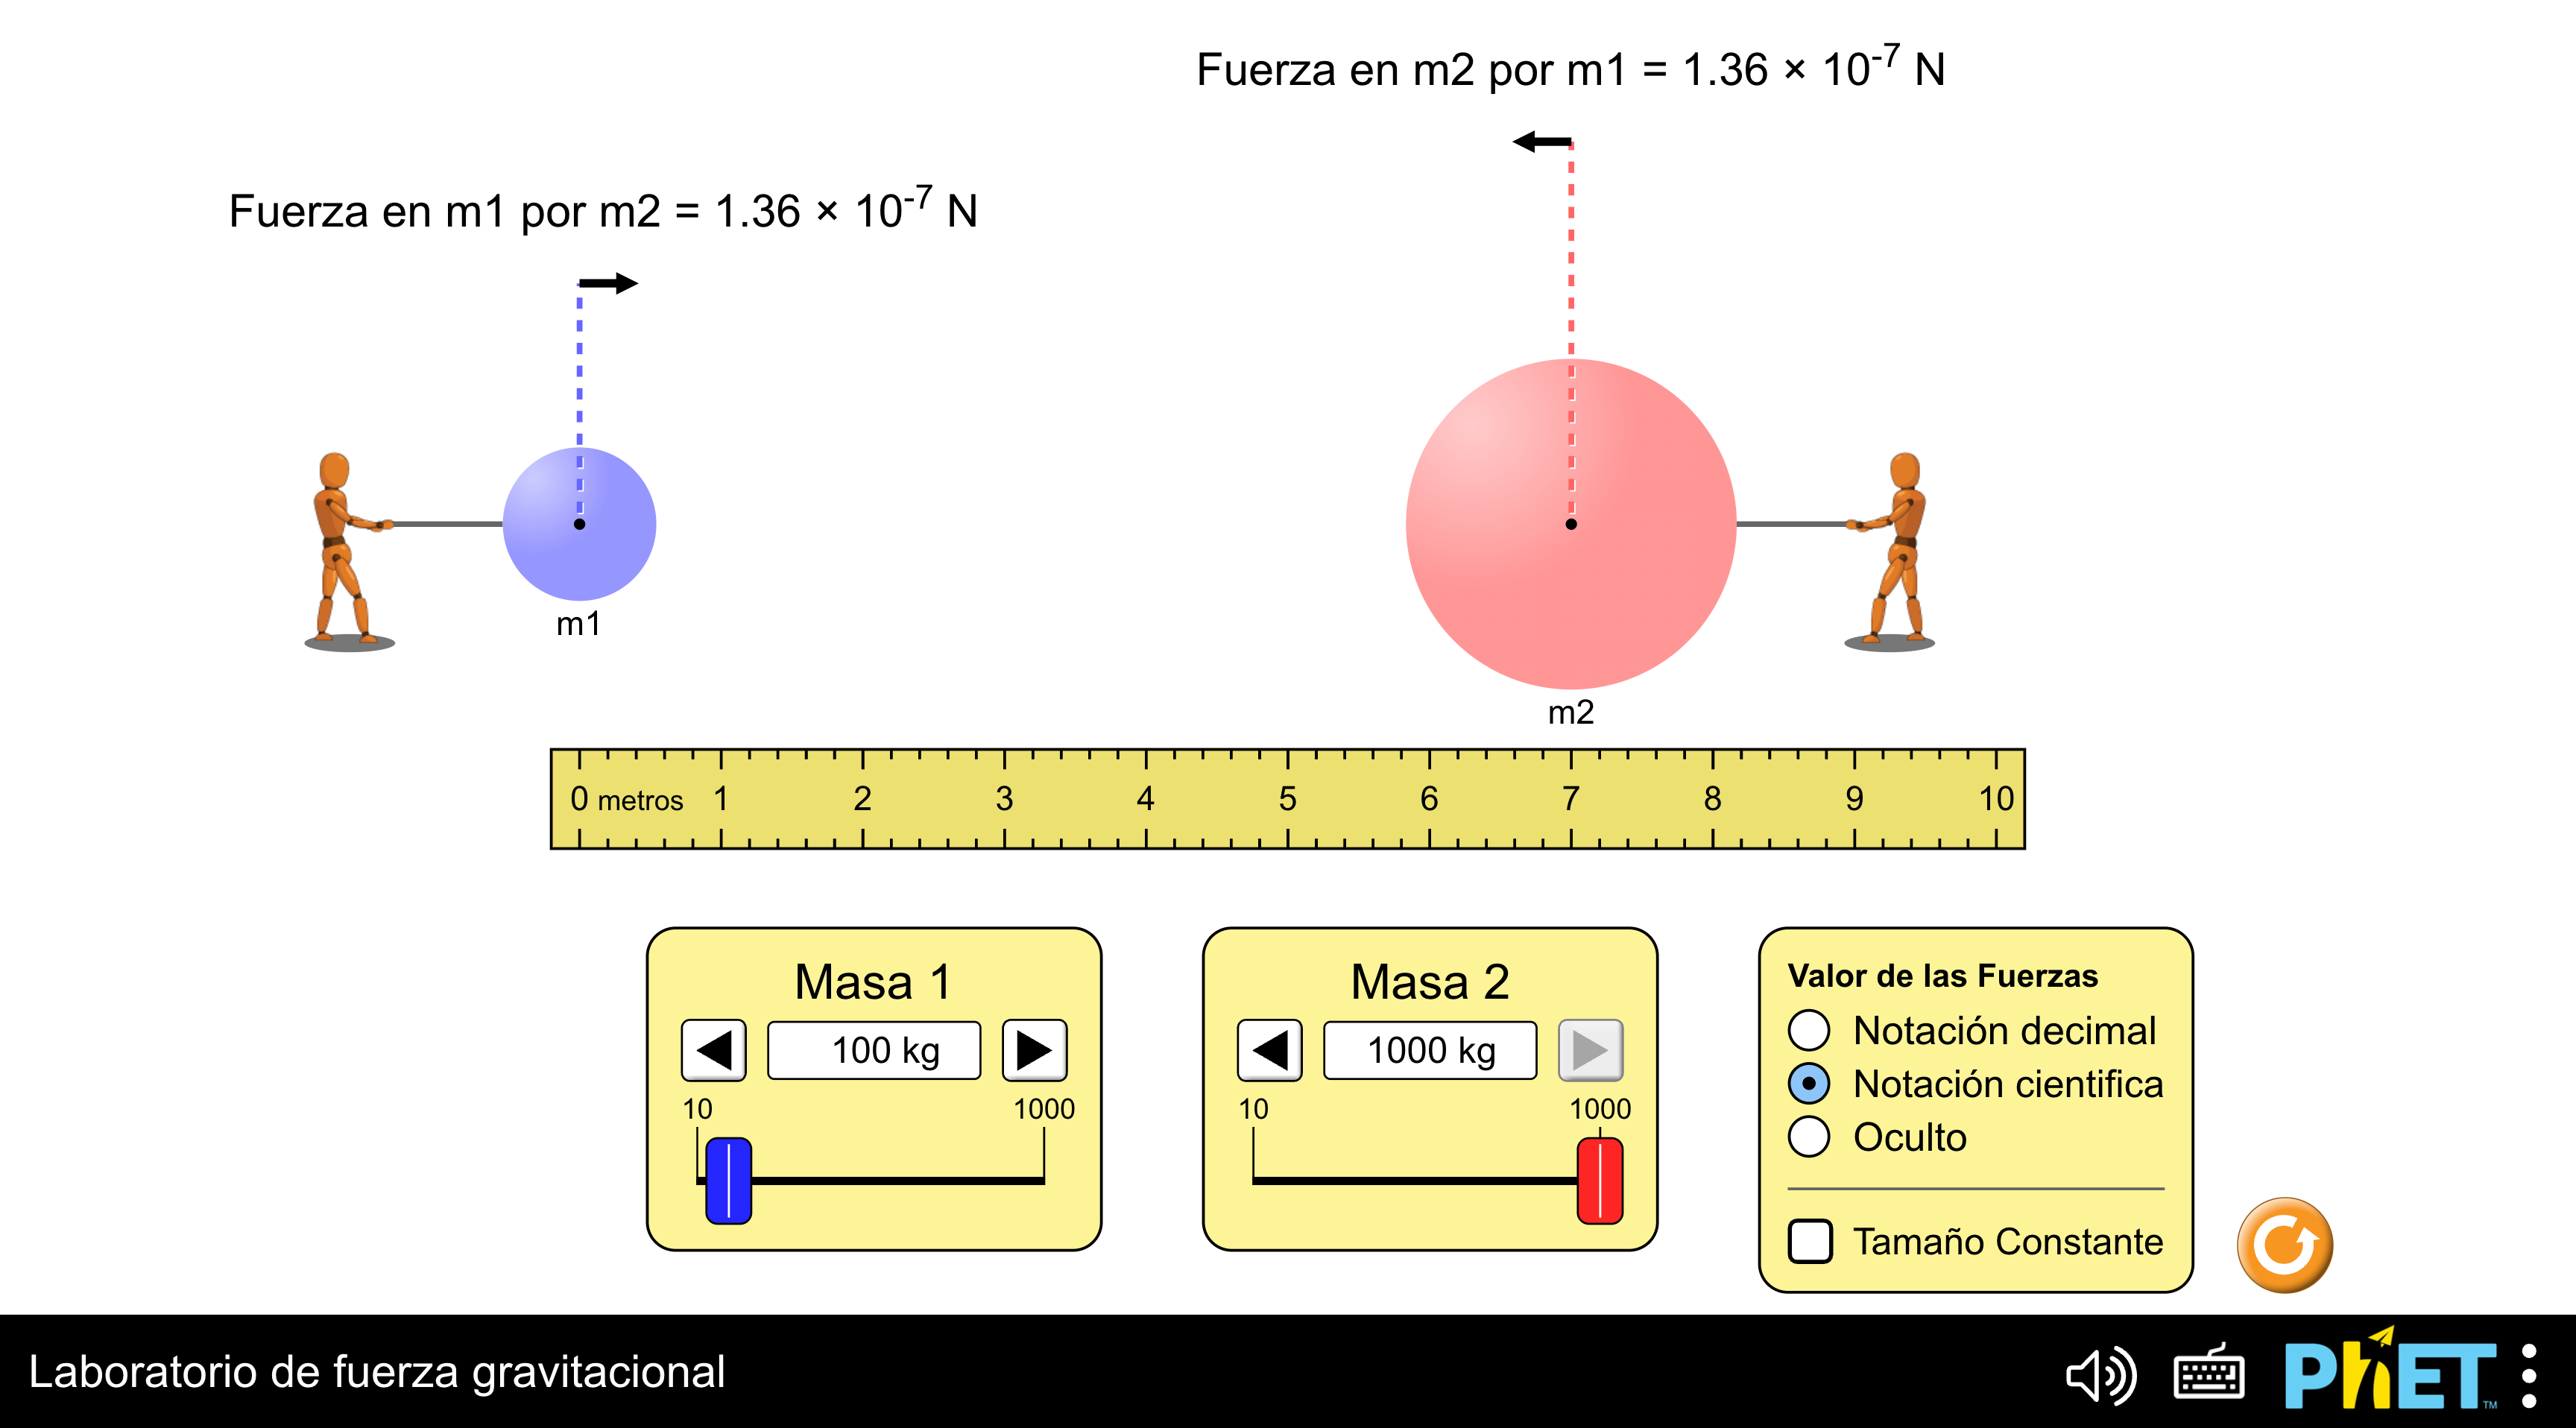
\includegraphics[width=1\linewidth]{m1_100_m2_1000_r_7.png}
    \caption{Masa 100 kg vs Masa 1000 kg, distancia de 7 m.}
\end{figure}

\begin{figure}[h]
    \centering
    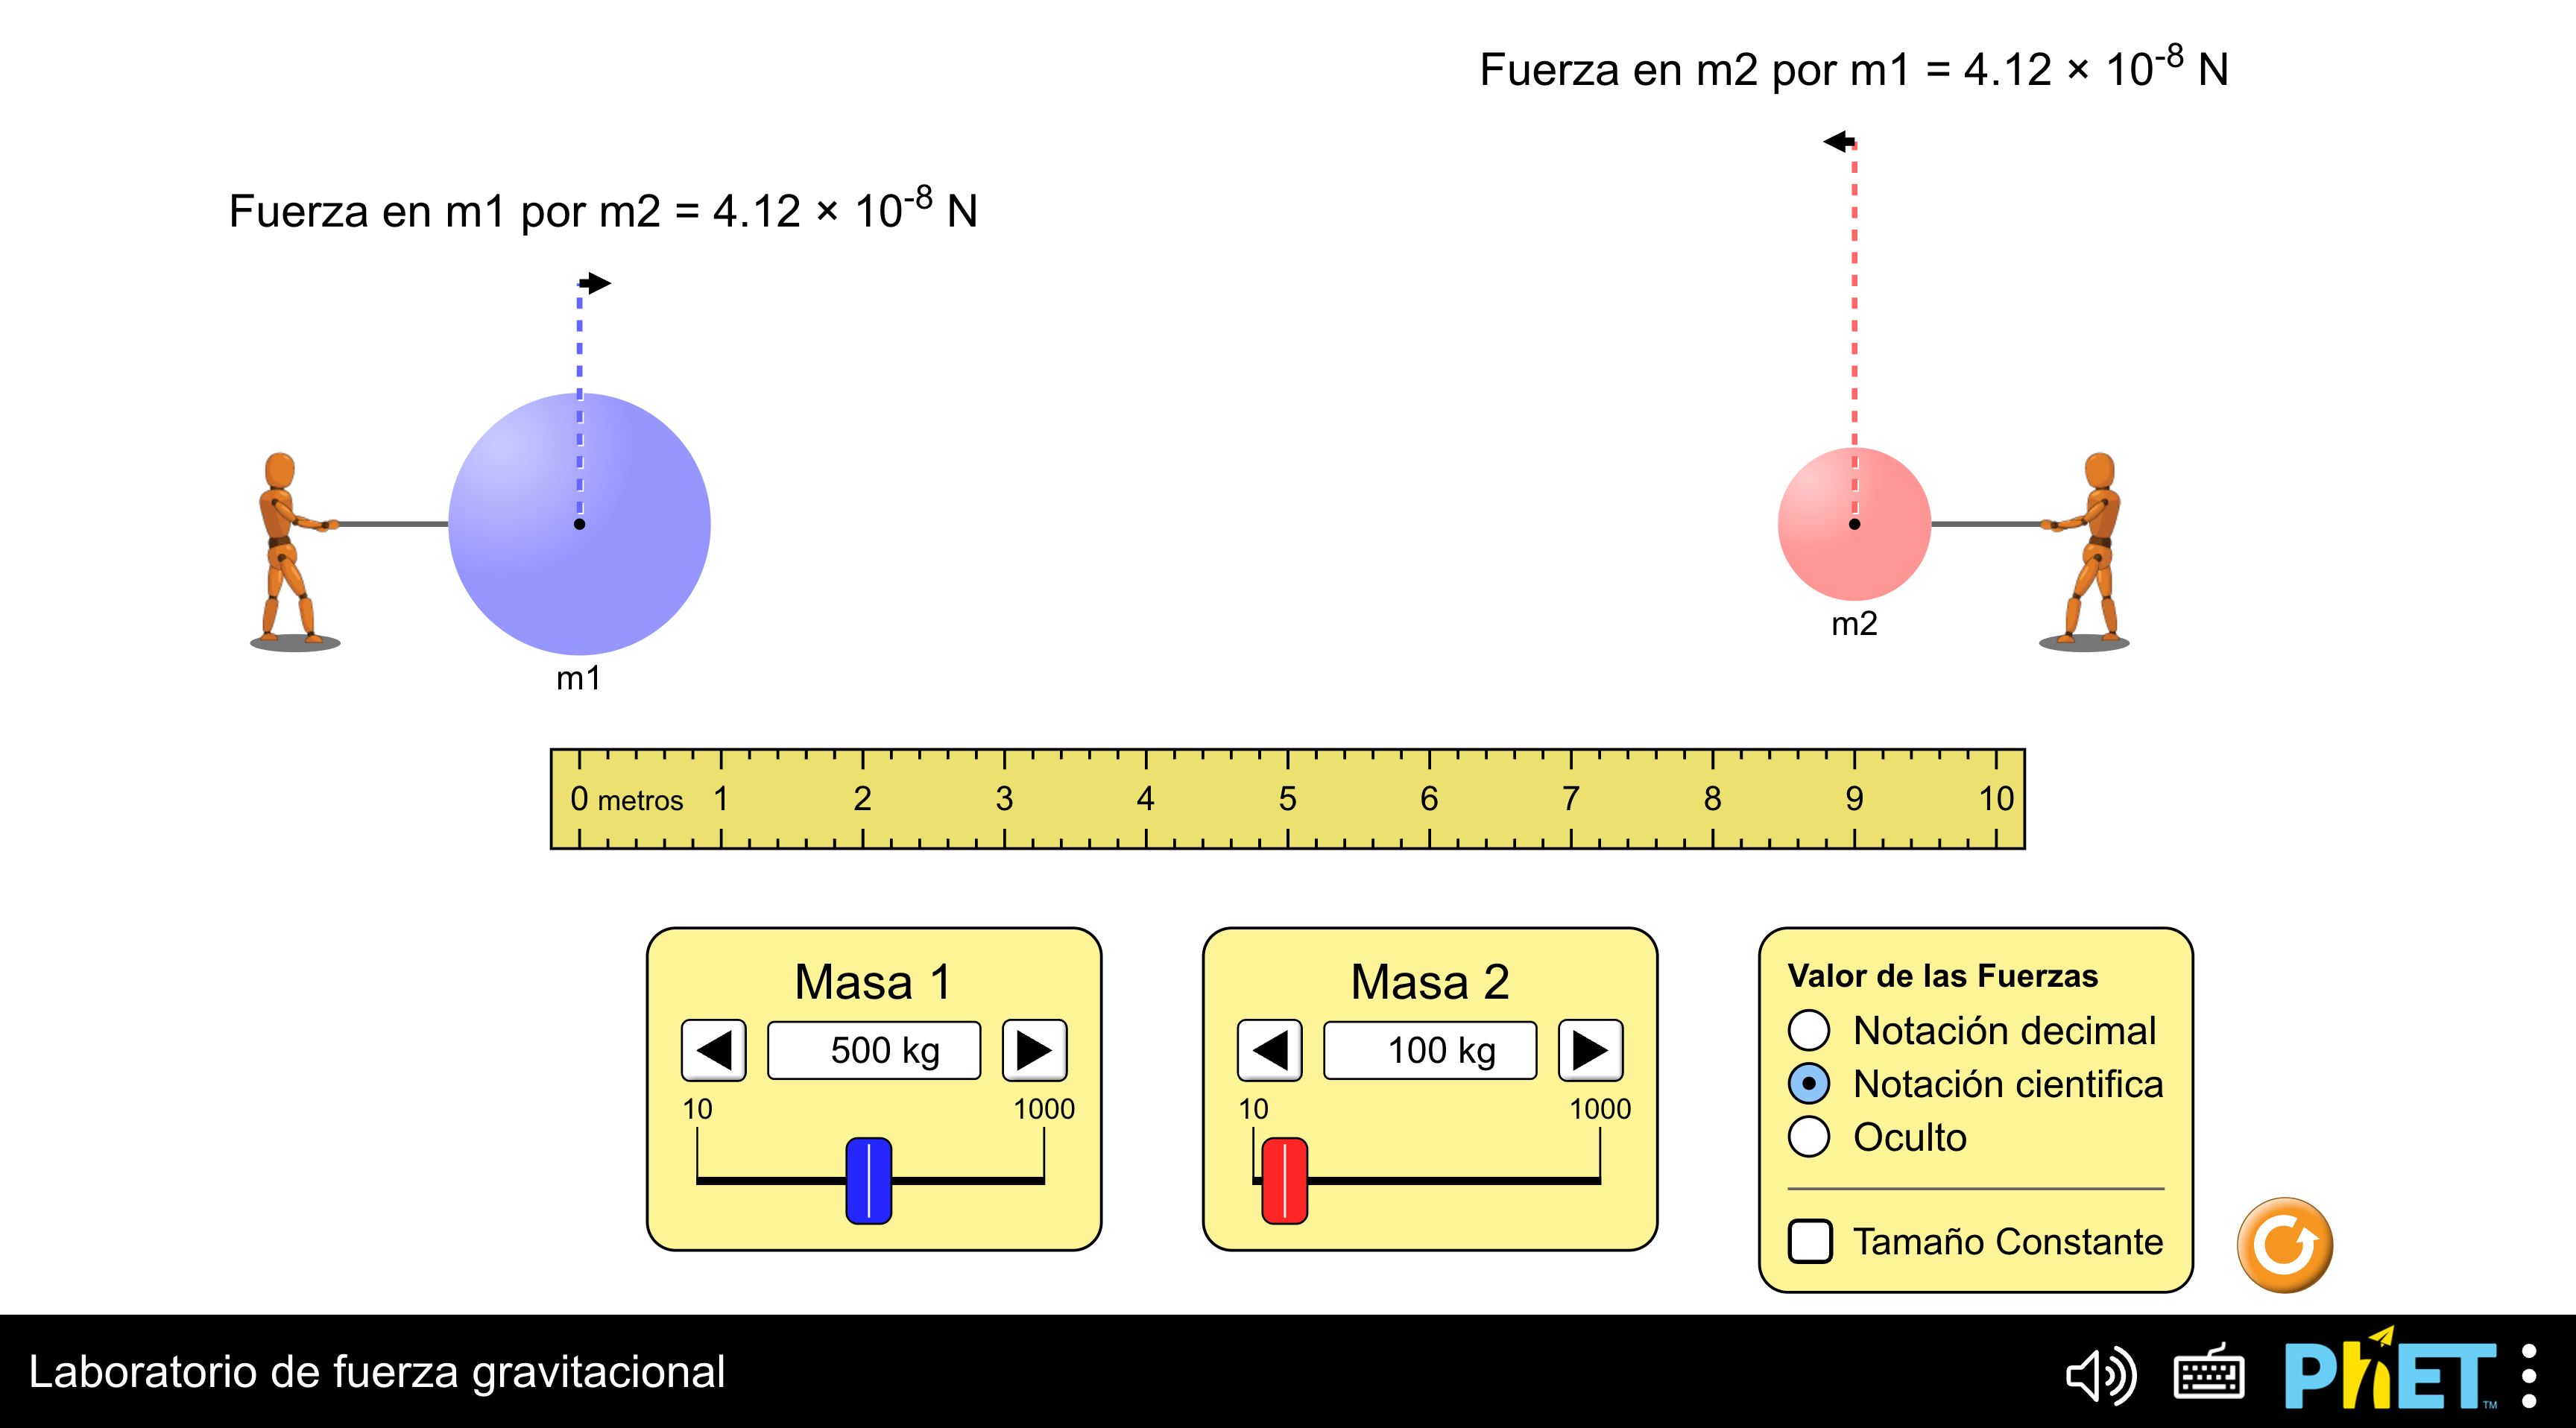
\includegraphics[width=1\linewidth]{m1_500_m2_100_r_9.png}
    \caption{Masa 500 kg vs Masa 100 kg, distancia de 9 m.}
\end{figure}

\begin{figure}[h]
    \centering
    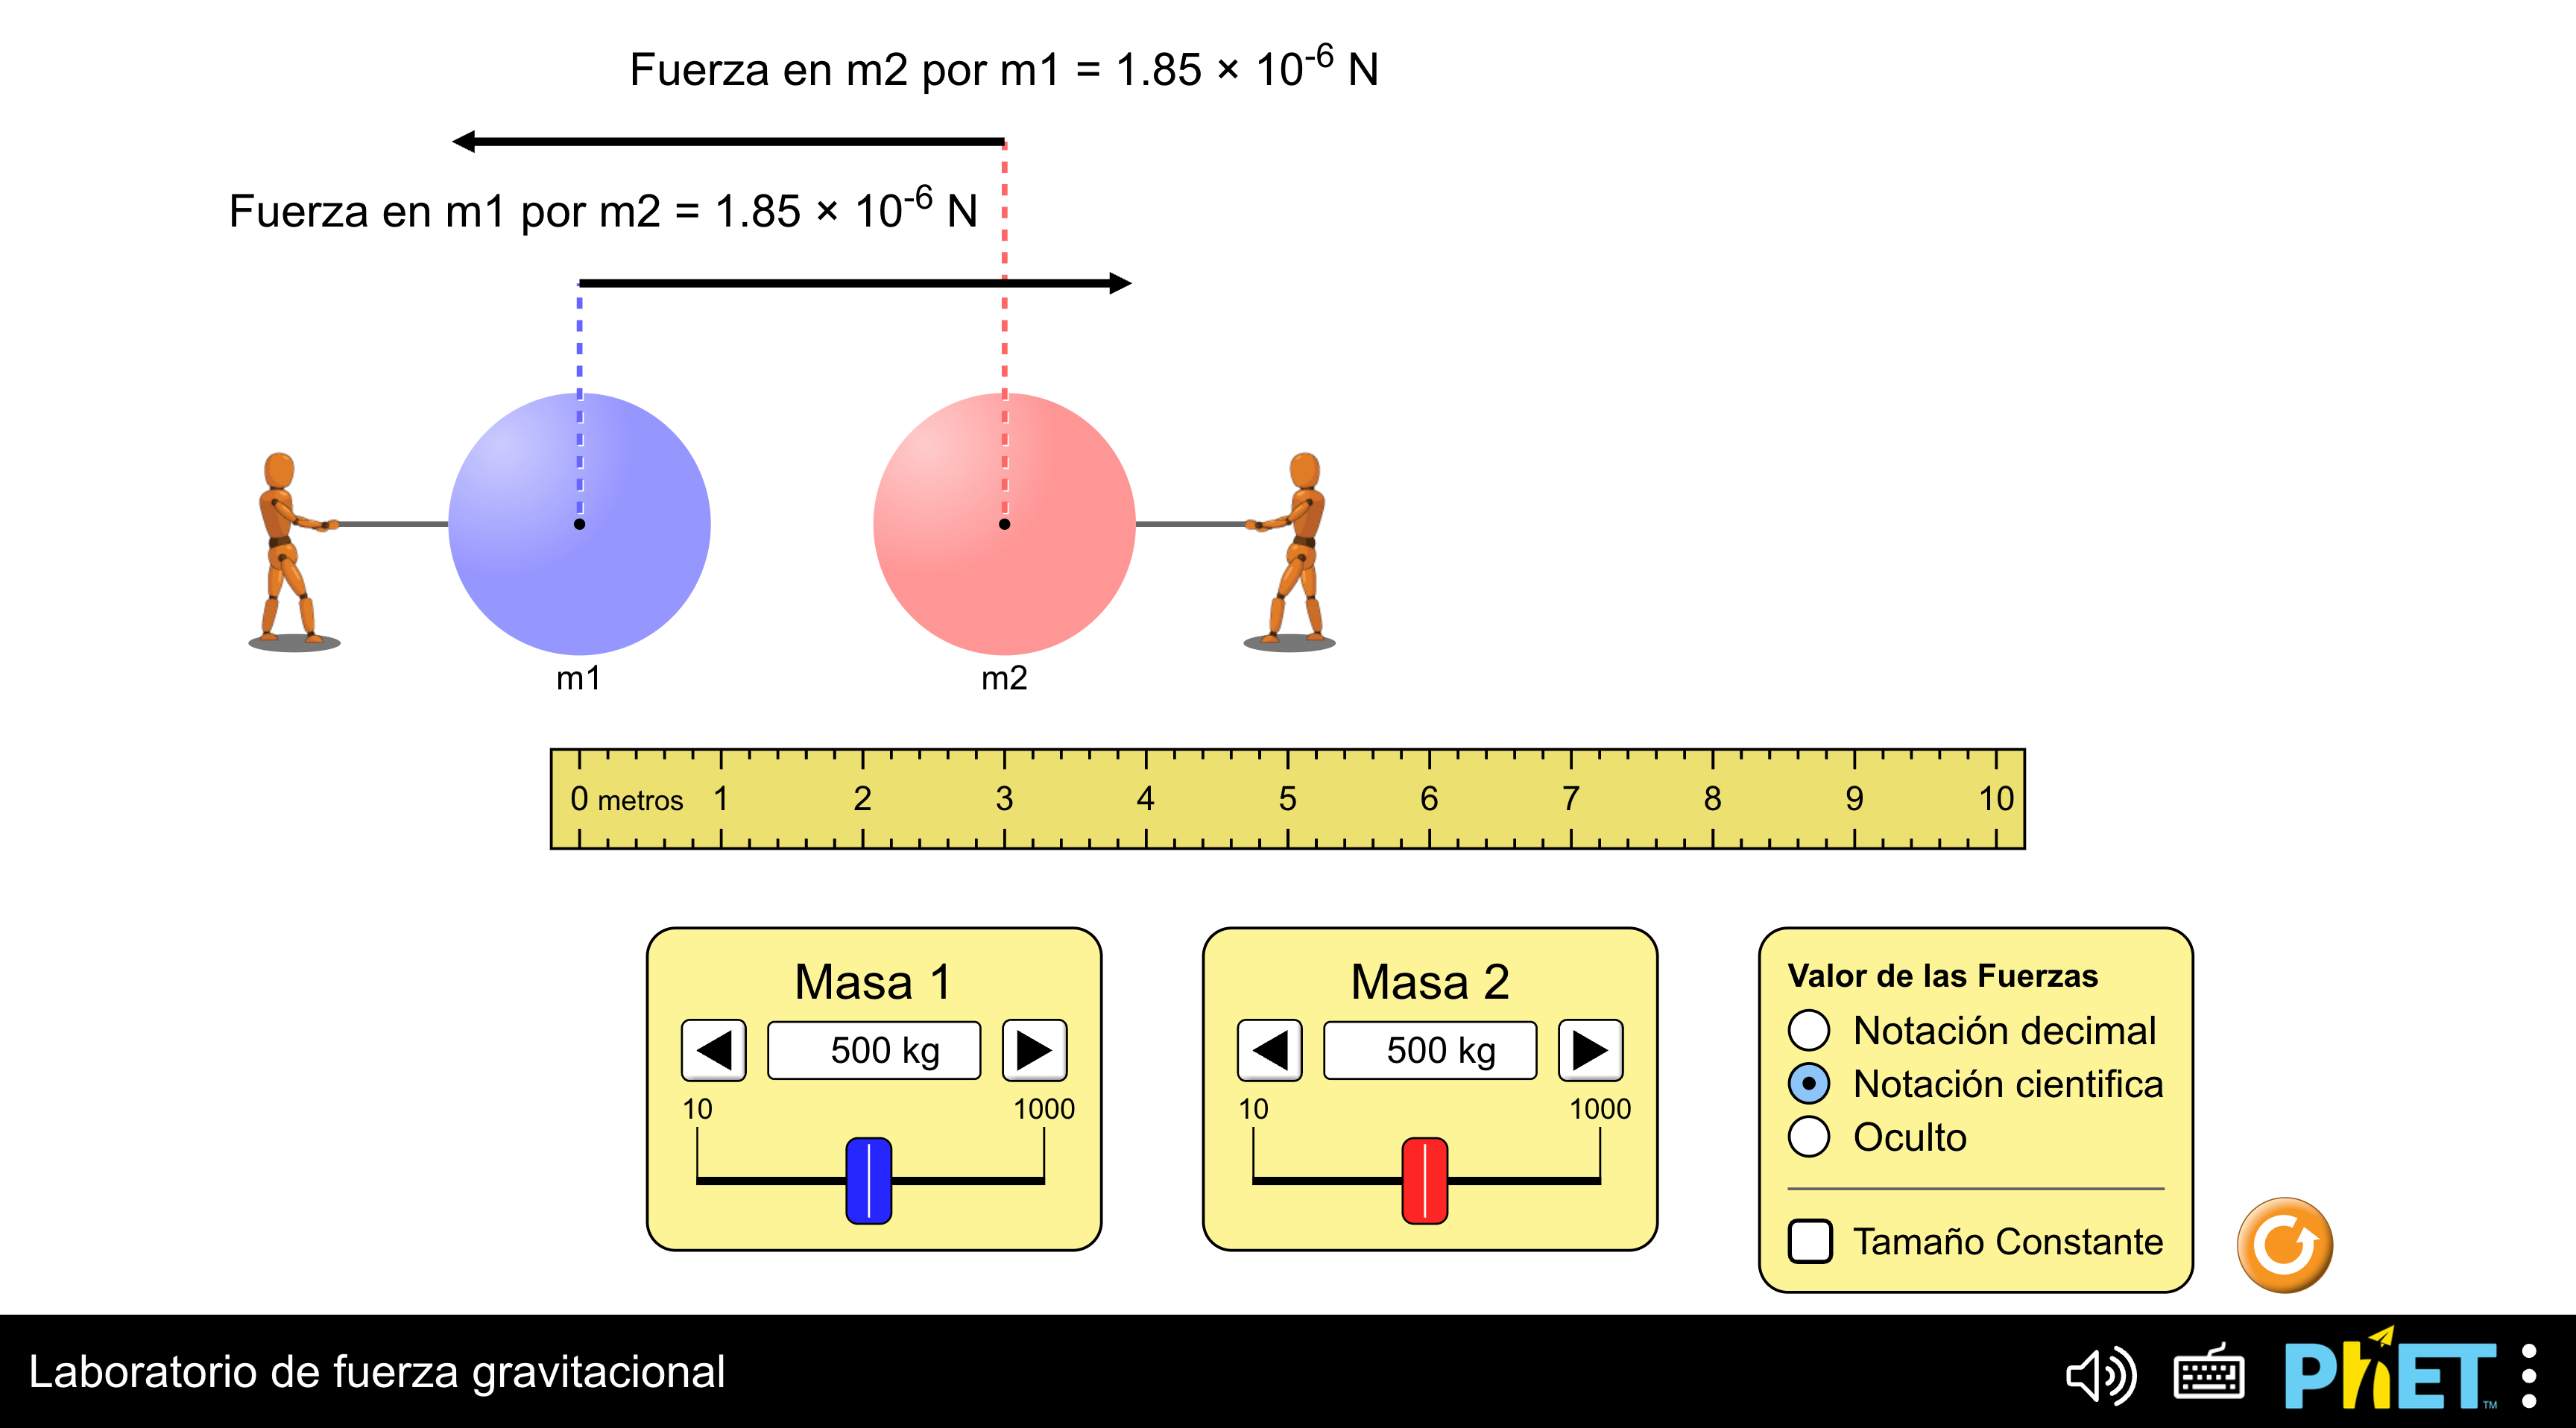
\includegraphics[width=1\linewidth]{m1_500_m2_500_r_3.png}
    \caption{Masa 500 kg vs Masa 500 kg, distancia de 3 m.}
\end{figure}

\begin{figure}[h]
    \centering
    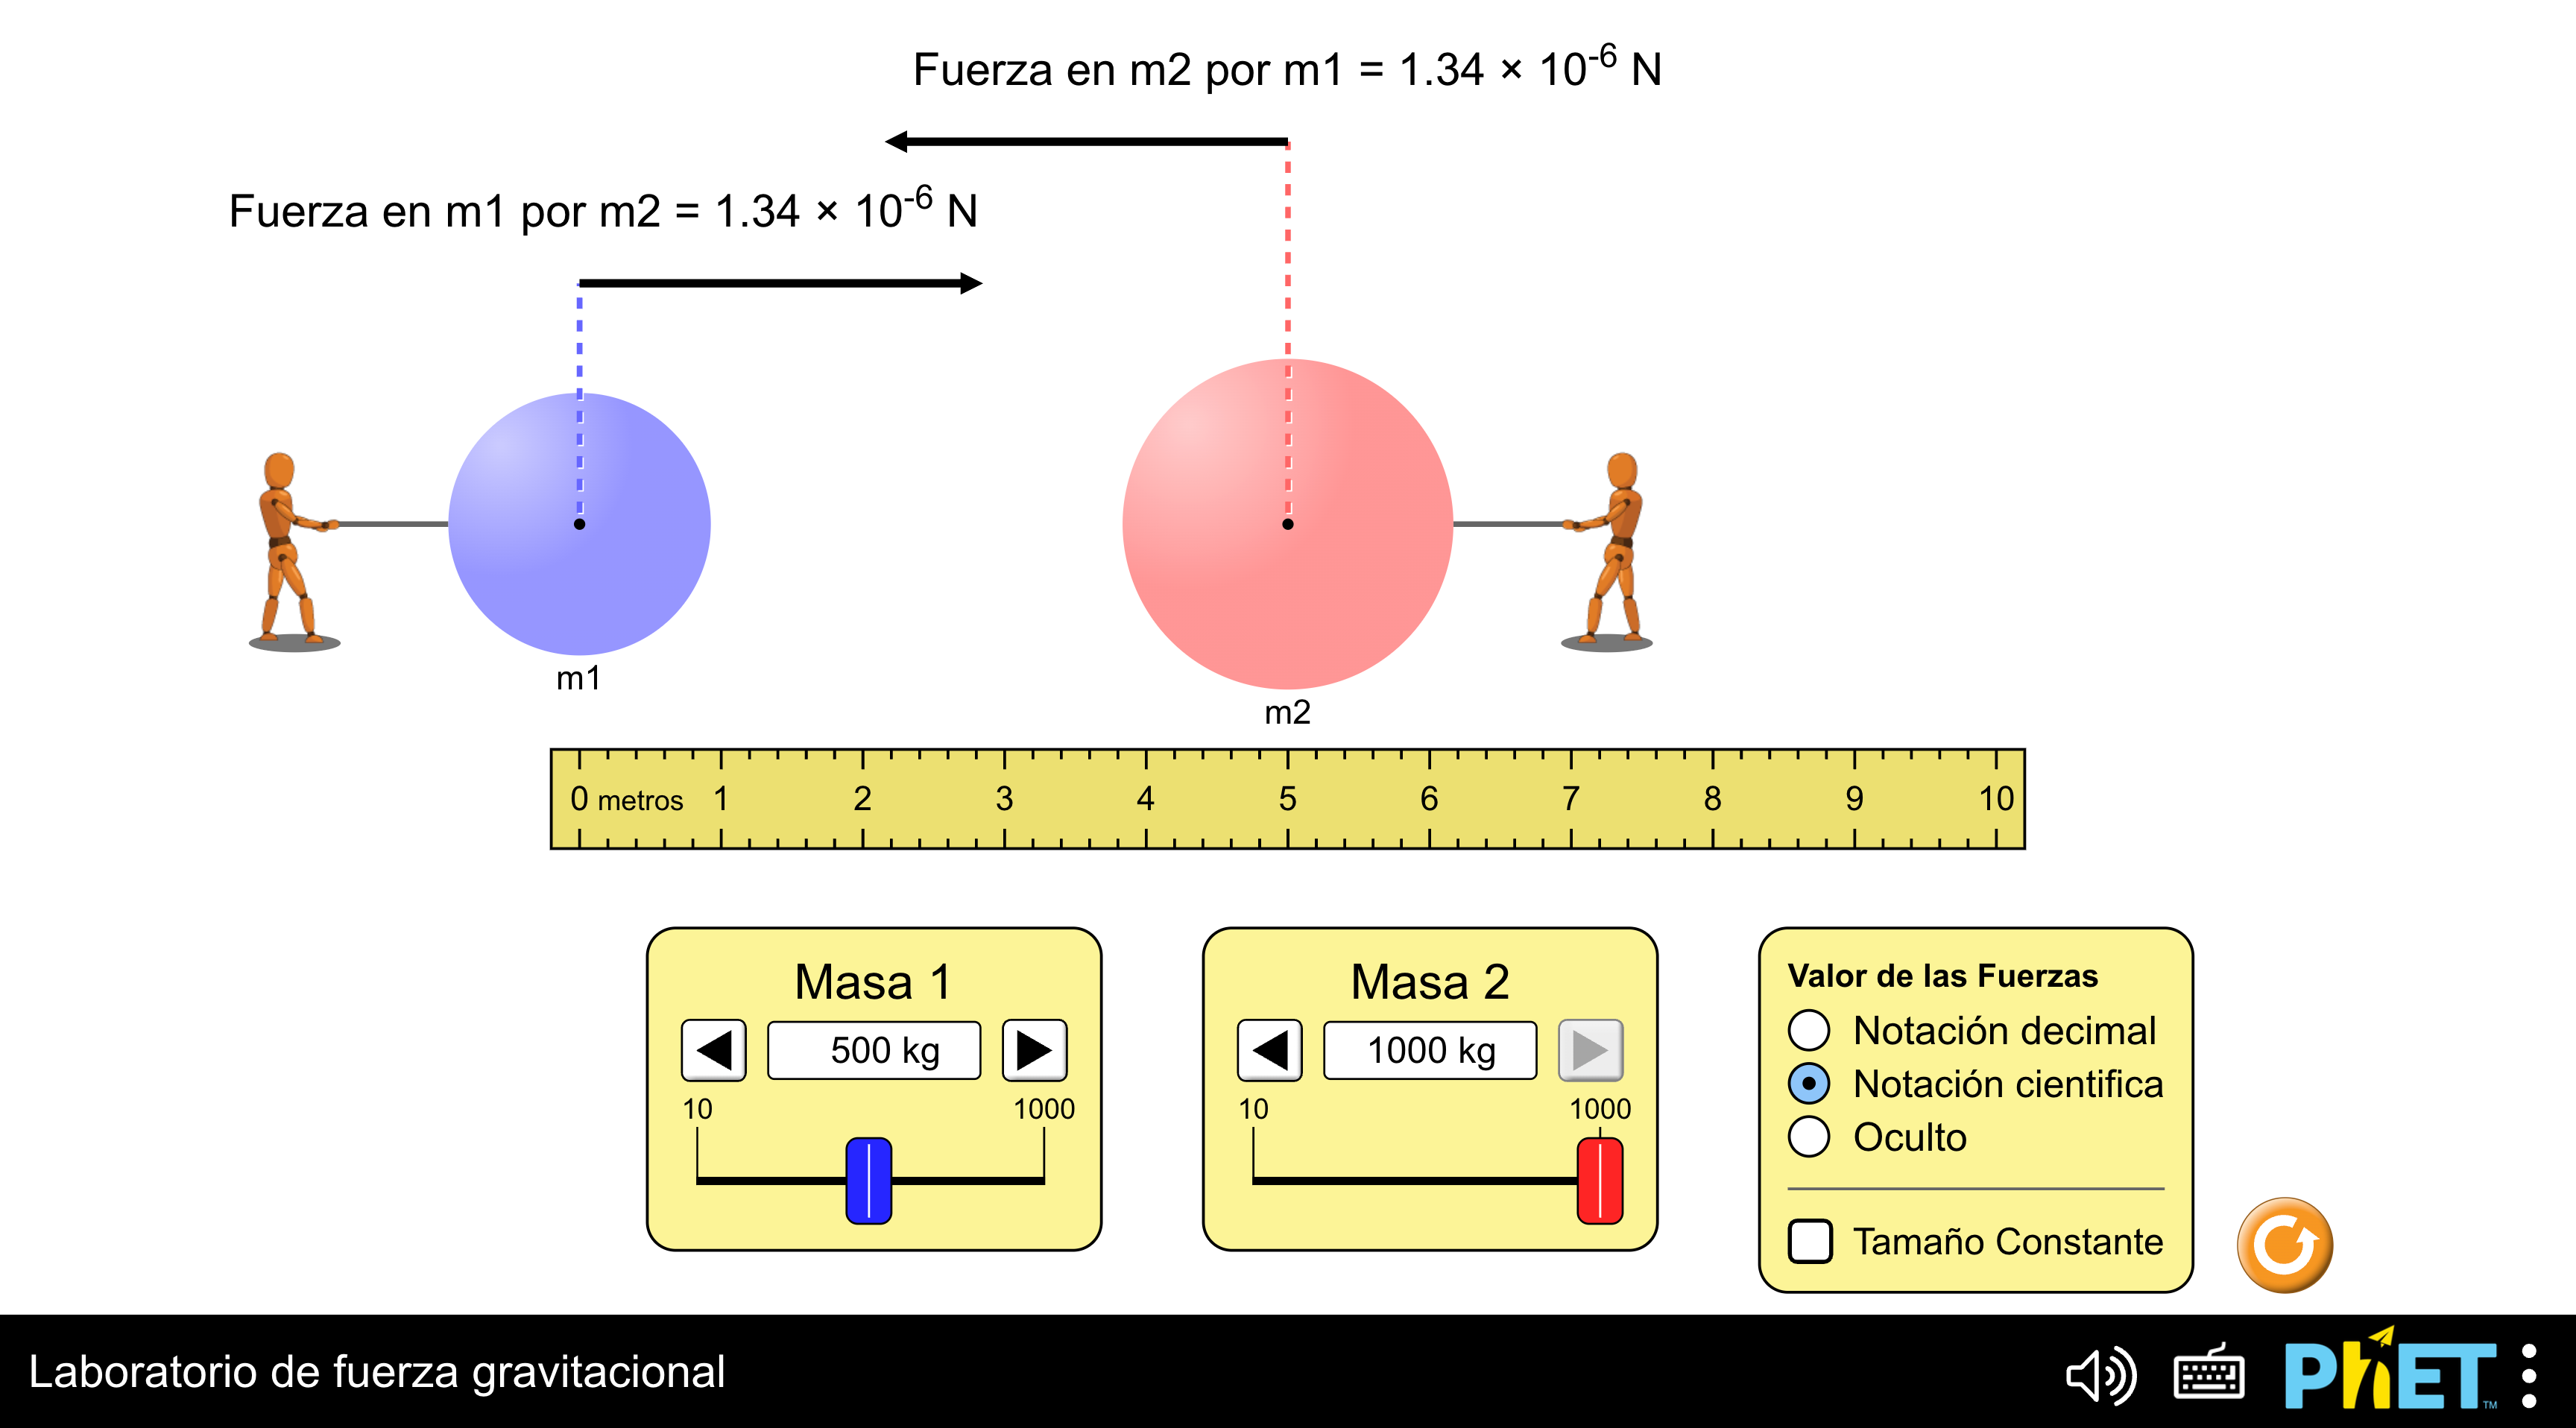
\includegraphics[width=1\linewidth]{m1_500_m2_1000_r_5.png}
    \caption{Masa 500 kg vs Masa 1000 kg, distancia de 5 m.}
\end{figure}

\begin{figure}[h]
    \centering
    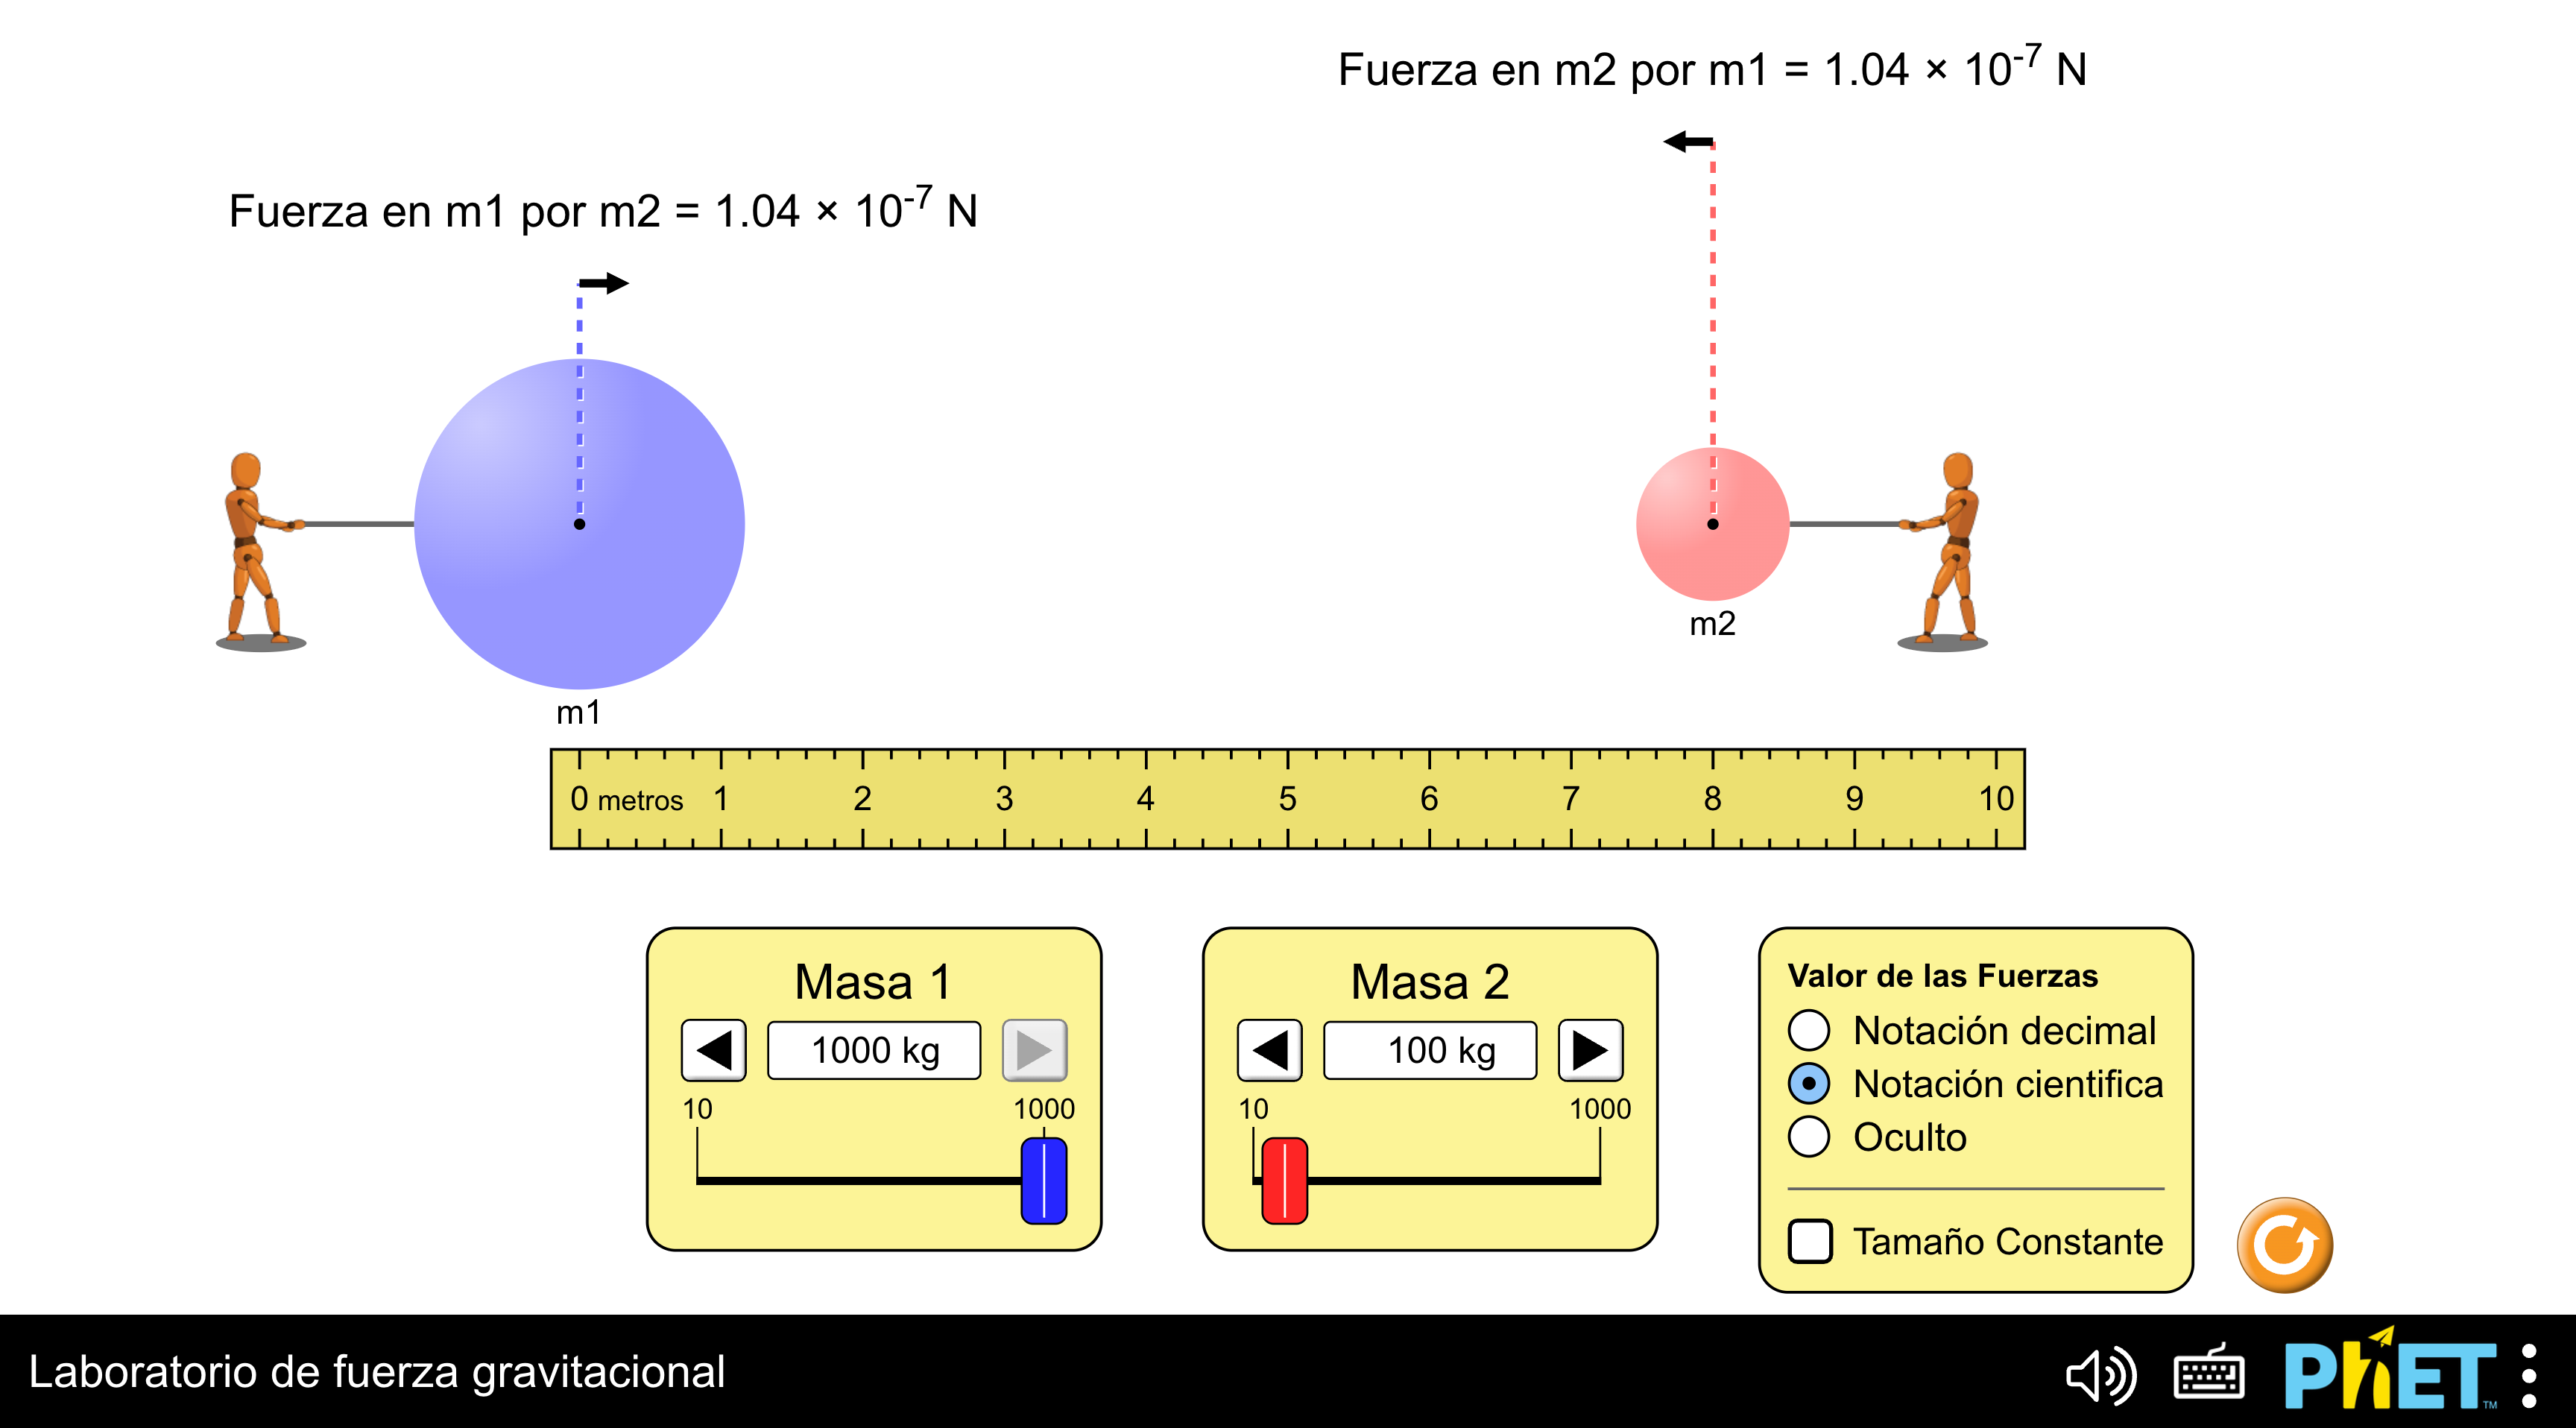
\includegraphics[width=1\linewidth]{m1_1000_m2_100_r_8.png}
    \caption{Masa 1000 kg vs Masa 100 kg, distancia de 8 m.}
\end{figure}

\begin{figure}[h]
    \centering
    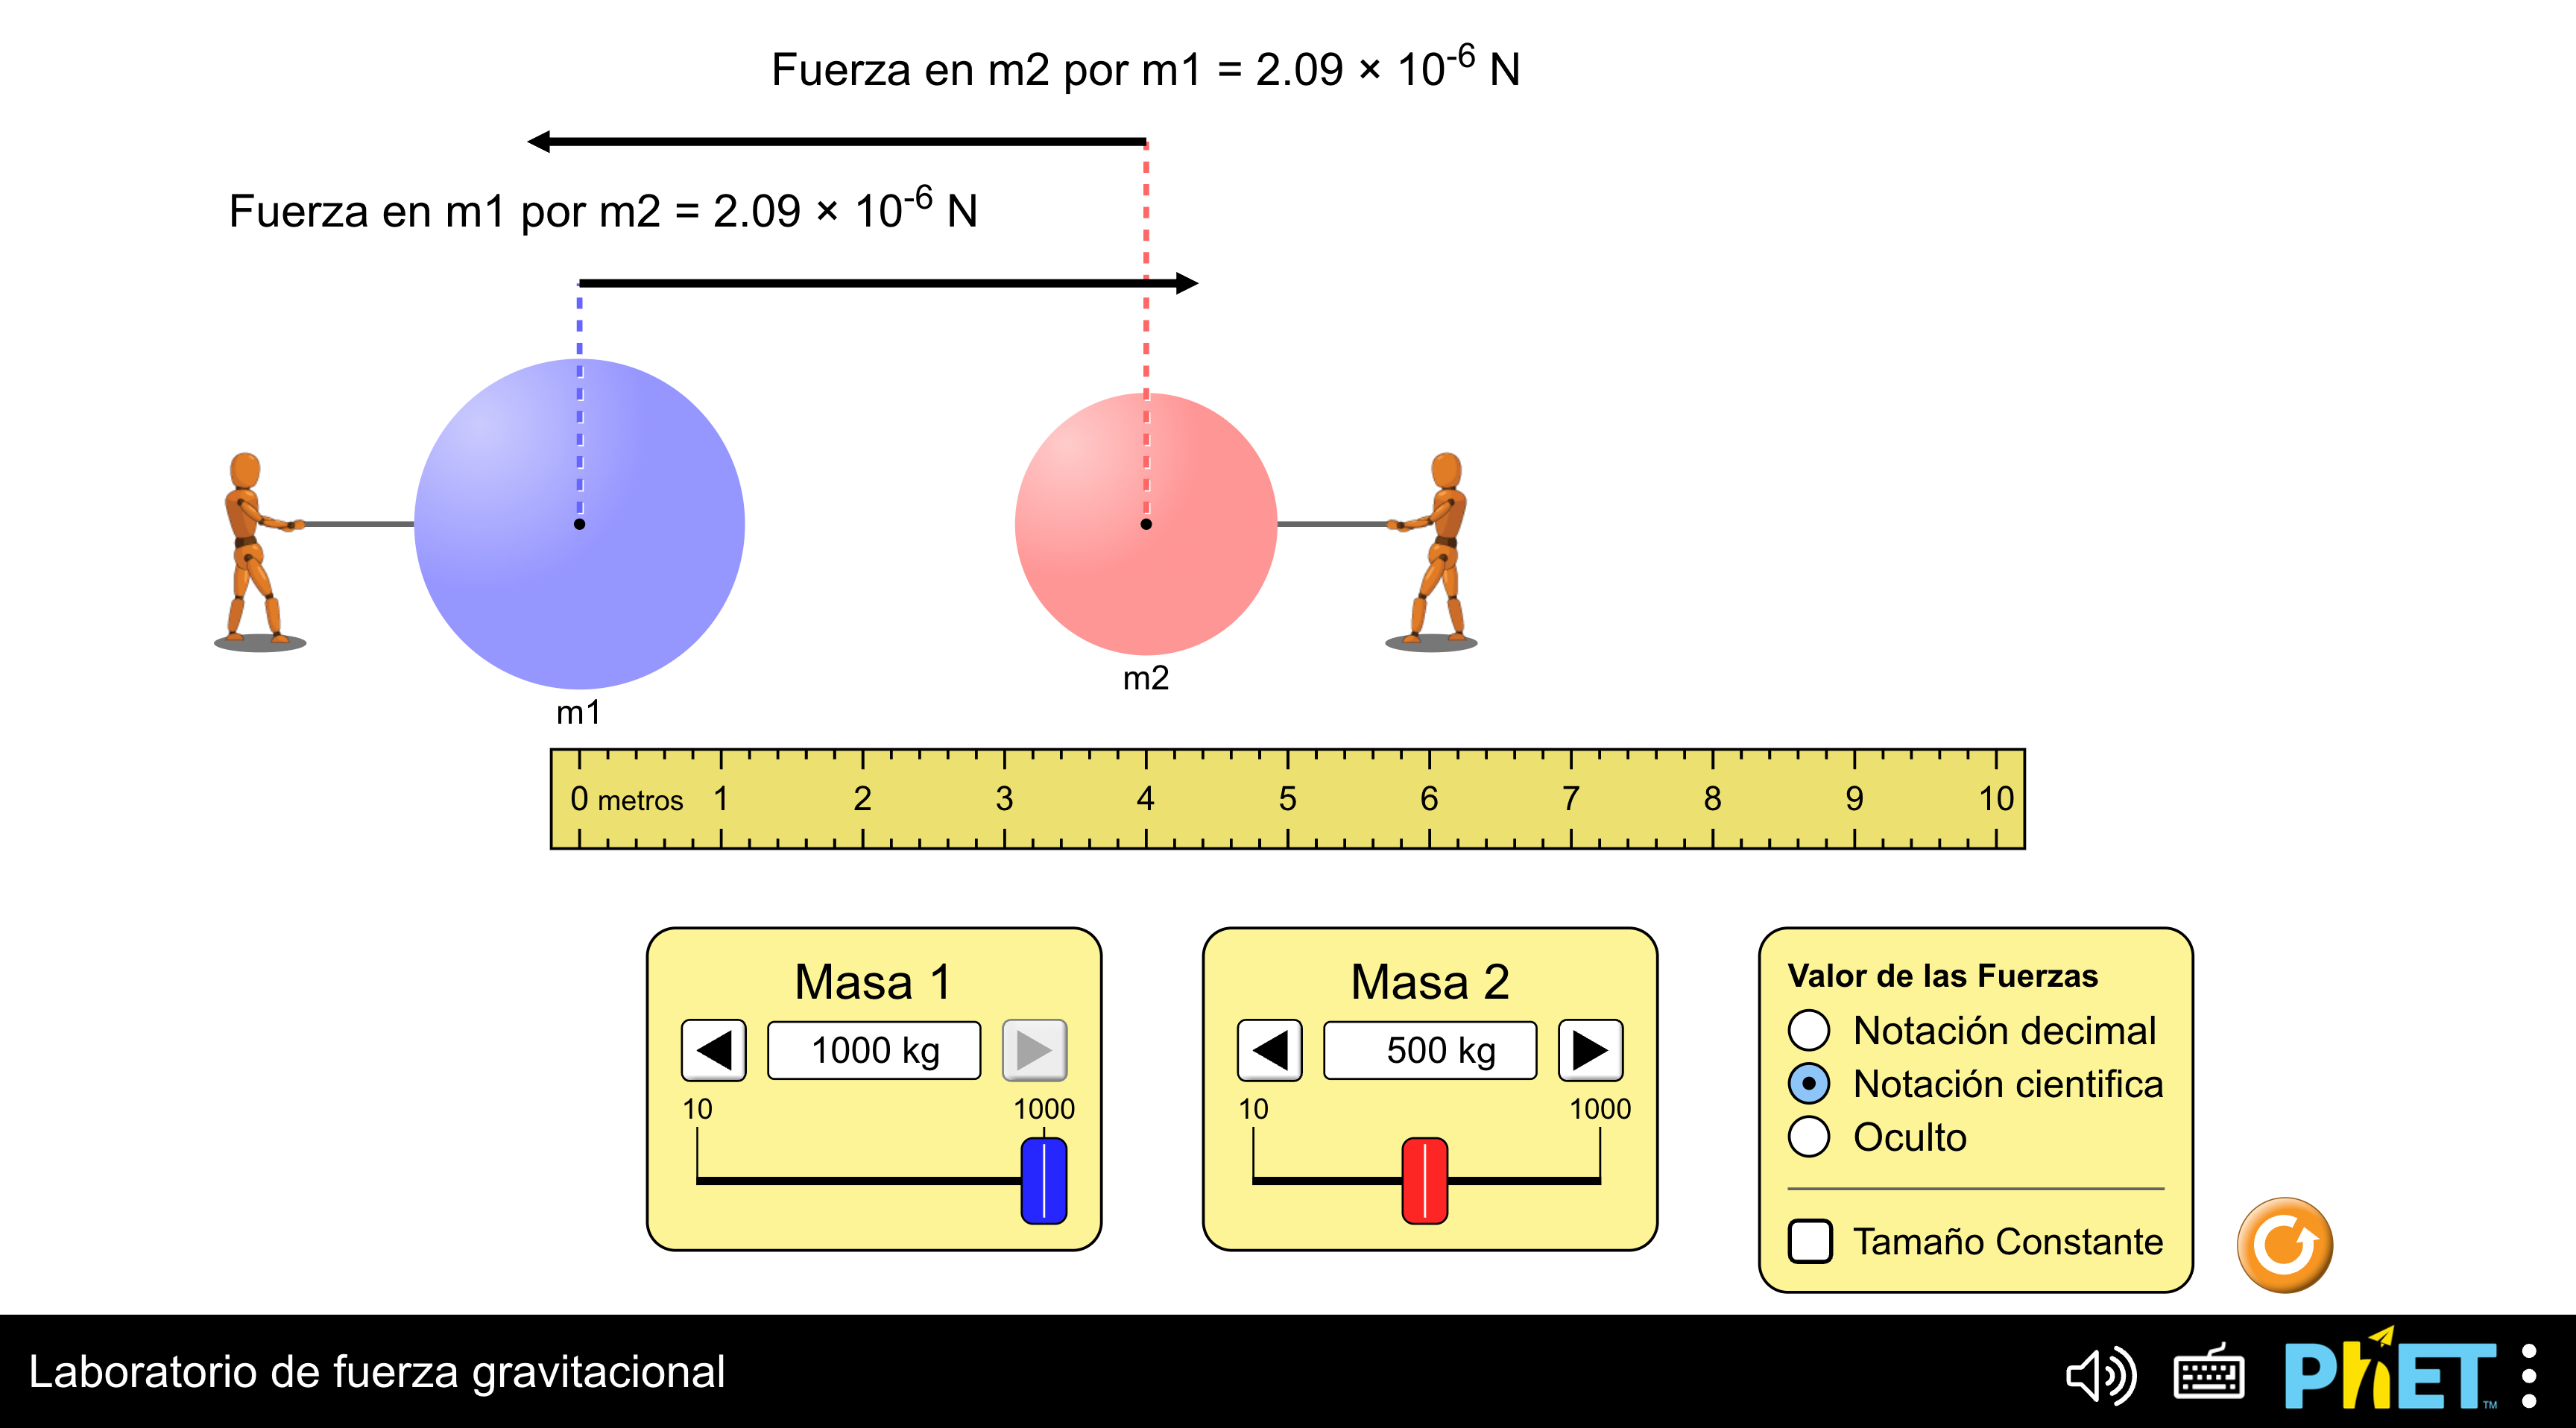
\includegraphics[width=1\linewidth]{m1_1000_m2_500_r_4.png}
    \caption{Masa 1000 kg vs Masa 500 kg, distancia de 4 m.}
\end{figure}

\begin{figure}[h]
    \centering
    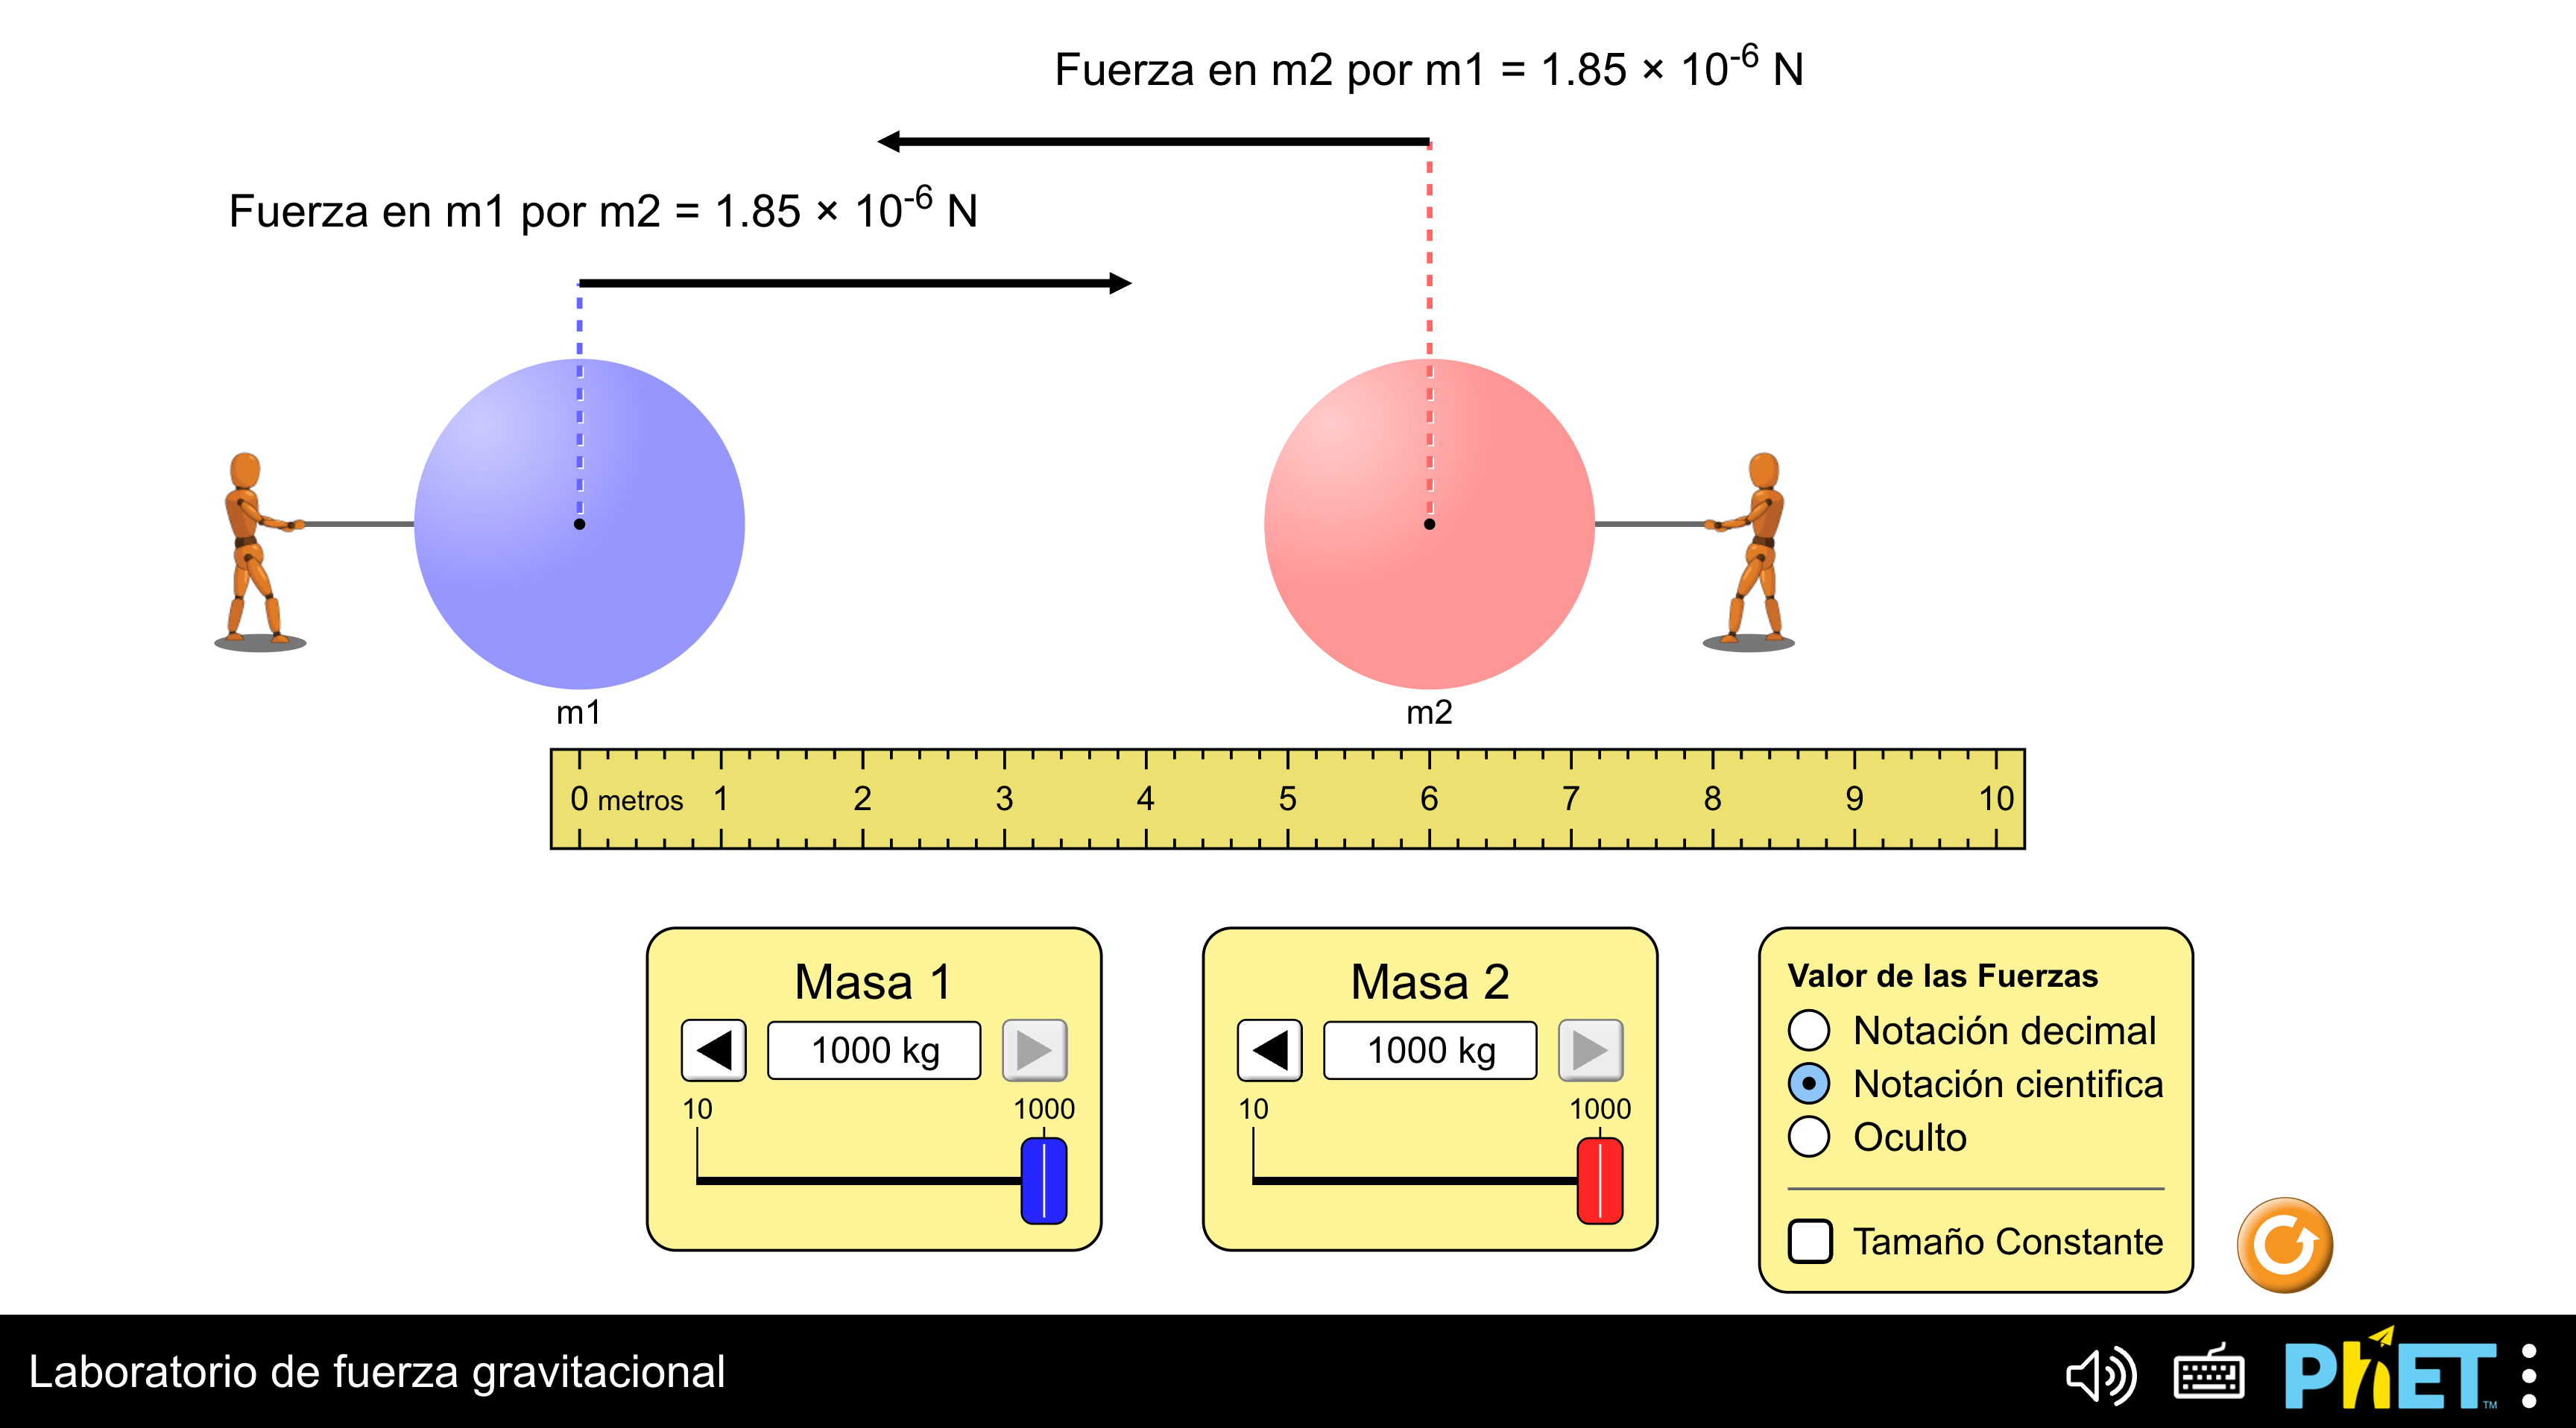
\includegraphics[width=1\linewidth]{m1_1000_m2_1000_r_6.png}
    \caption{Masa 1000 kg vs Masa 1000 kg, distancia de 6 m.}
\end{figure}

\end{document}
